% gjilguid2e.tex
% V2.0 released 1998 December 18
% V2.1 released 2003 October 7 -- Gregor Hutton, updated the web address for the style files.

\documentclass[extra]{gji} %referee, mreferee
\usepackage{timet}
%\usepackage{float}
\usepackage[pdftex]{graphicx}
\usepackage{subcaption}
\usepackage{setspace}
\usepackage{url}
%% Math or theory people may want to include the handy AMS macros
\usepackage{amssymb}
\usepackage[fleqn]{amsmath}
\usepackage{amsfonts}
\usepackage{algorithm}
\usepackage{algorithmicx}
%\usepackage{textcomp}
% "\nl means \newline" is in conflict with algorithm2e
\let\nl\undefined
\usepackage[linesnumbered, algoruled, lined, commentsnumbered,algo2e]{algorithm2e}
\usepackage{algpseudocode}
%\usepackage[pdftex,pdfpagelabels,bookmarks,hyperindex,hyperFigs]{hyperref}

% Users can choose between the Low Resolution Fig. folder ./Fig/LowRes/ (faster) or the High Resolution Fig. folder ./Fig/HighRes/
% \graphicspath{ {./Fig/LowRes/} }

% An example of defining macros
%\newcommand{\rs}[1]{\mathstrut\mbox{\scriptsize\rm #1}}
%\newcommand{\rr}[1]{\mbox{\rm #1}}
%\usepackage{rotating}
% \usepackage{array}
% \newcolumntype{P}[1]{>{\centering\arraybackslash}p{#1}}

% \title[A framework for petrophysically and geologically guided inversion]
%   {A framework for petrophysically and geologically guided geophysical inversion using a dynamic Gaussian mixture model prior}
% \author[Thibaut Astic and Douglas W. Oldenburg]
%   {Thibaut Astic$^1$ and Douglas W. Oldenburg$^1$\\
%   $^1$ Geophysical Inversion Facility, University of British Columbia, Vancouver, BC, Canada
%   }
% \date{December 2019}
% \pagerange{1989--2012}
% \volume{219}
% \pubyear{2019, Issue 3}

% Authors with AMS fonts and mssymb.tex can comment out the following
% line to get the correct symbol for Geophysical Journal International.
\let\leqslant=\leq

\newtheorem{theorem}{Theorem}[section]

\begin{document}
\eqsecnum

\label{firstpage}

\maketitle

\begin{abstract}
We propose a new framework for incorporating petrophysical and geological information into voxel-based geophysical inversion. By developing the geophysical inverse problem from a probabilistic perspective, we redesign the objective function and the iteration steps as a suite of cyclic optimization problems in which three separate MAP optimization problems are solved using geophysical, petrophysical and geological data respectively. By quantitatively linking these data into a single framework, we recover a final inverted model that reproduces the observed, or desired, petrophysical and geological features while fitting the geophysical data. To achieve our goal we replace the Gaussian prior, used in the Tikhonov inversion approach, by a Gaussian mixture model. After each geophysical model update, the mixture parameters (means, variances and proportions) are determined by the geophysical model and the expected characteristics of the lithologies through another optimization process using the Expectation-Maximization algorithm. We then classify the model cells into rock units according to the petrophysical and geological information. These two additional steps over the petrophysical and geological data result in a dynamic update of the reference model and associated weights and guide the inversion towards reproducing the expected petrophysical and geological characteristics. The resulting geophysical objective function does not require extra terms to include the additional petrophysical and geological information; this is an important distinction between our work and previous frameworks that carry out joint geophysical and petrophysical data inversion. We highlight different capabilities of our methodology by inverting magnetotelluric and DC resistivity data in 1D and 2D respectively. Finally we apply our framework to inverting airborne frequency domain data, acquired in Australia, for the detection and characterization of saline contamination of freshwater.
\end{abstract}

\begin{keywords}
Inverse theory -- Joint Inversion -- Clustering -- Electrical properties -- Non-linear electromagnetics -- Probability distributions
\end{keywords}

%%%%%%%%%%%%%%%%%%%%%%%%%%%%%%%%%%%%%%%%%%%%%%%%%%%%%%%%%%%%%%%%%%%%%%%%%%%%%%%
\section{Introduction}

Geophysical inversions are an essential tool for mapping the subsurface. However, the image of the underground retrieved from an inversion rarely benefits from the full range of knowledge because petrophysical relationships or expected geologic features are not easily incorporated into traditional geophysical inversions. Since the early 2000's, there has been an increasing interest in including this information to obtain more realistic geological interpretations \citep{Linde2015,Moorkamp2016}. Various strategies have been implemented such as adding bound constraints and preferential trends \citep{Astic2018,Lelievre2009,Li2000,Williams_2008}, parameterization of the expected shapes of the geological bodies \citep{Fullagar2008,McMillan2015}, inclusion of more complex non-geophysical data such as structural data \citep{Wu2017}, reproducing petrophysical data \citep{Bosch2009,Grana2010,Sun2015,Zhdanov} and training on geological images \citep{Lochbuhler2015}.

For the inclusion of petrophysical data, the most recent frameworks have focused on using clustering techniques such as the fuzzy C-means algorithm. This was first used in \cite{Paasche2007} and later expanded in \cite{Lelievre2012}. This approach adds a clustering term to the objective function and allows a less strict relationship between the physical properties of interest. Further expansion of the method has been carried out by \cite{Sun2015, Sun2016, Sun2017}. In addition to the fuzzy C-means clustering term, they added an iterative update to the cluster centers; this starts to introduce the notion of uncertainty for the petrophysical data.
For linear problems, \cite{Grana2017} proposed a Bayesian formulation using a fixed Gaussian mixture model as prior, which allows them to estimate the posterior distribution and then to sample from that distribution.
\cite{Giraud2017} on their side focused on reducing geological uncertainties by linking geophysical inversion and stochastic geological modeling through petrophysical information using a fixed Gaussian mixture model to model the petrophysical information. They modified the usual least-squares objective function of the geophysical inverse problem by adding a probabilistic term, computed from the prior petrophysical and geological distributions. To do this they required fixed, and thus very strong, priors for both the petrophysical and geological information. That information however is not often well-known and may exist only at a qualitative level.

\begin{figure}
    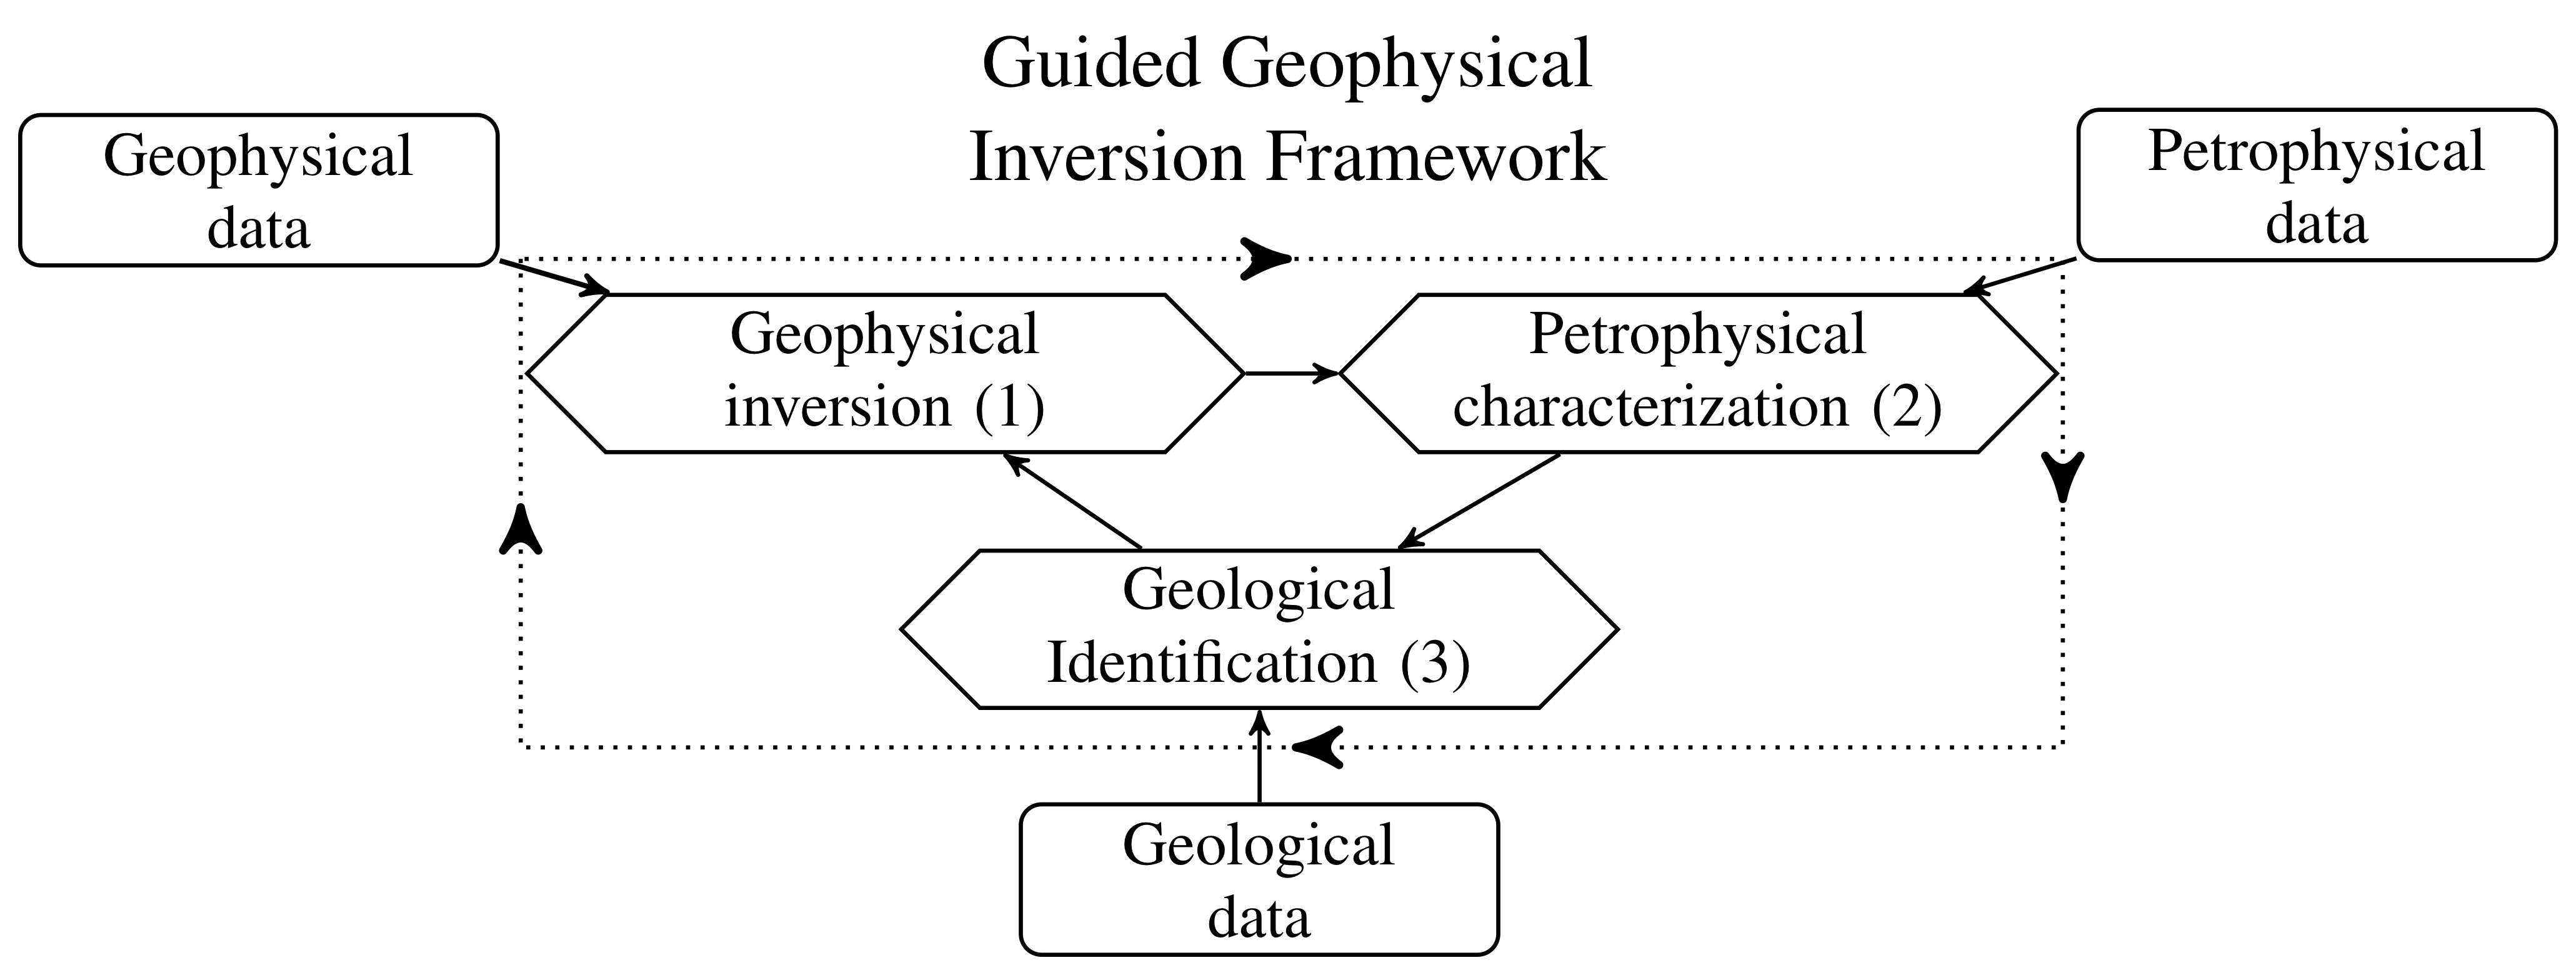
\includegraphics[width=\columnwidth]{./Fig/LowRes/Framework_with_numbers.png}
    \caption{A graphical representation for our framework. Each diamond is a MAP estimation which requires data (shown in rectangular boxes) as well as input from the other MAP estimates.
    }
    \label{graph_simple}
\end{figure}

This paper presents a new framework for petrophysically and geologically guided inversion (PGI) that generalizes concepts presented in \cite{Grana2017}, \cite{Giraud2017} and \cite{Sun2015}. We use a Gaussian mixture model (GMM) that represents our petrophysical and geological knowledge to regularize the geophysical inversion; this is analogous to the approach used by \cite{Grana2017}. The idea of learning the physical properties mean values described in \cite{Sun2015} is formalized and extended to the variances and proportions of the GMM.  At the same time we are able to include the geological information in the GMM in a similar way as did \cite{Giraud2017}.

Our algorithm involves three optimization problems (Fig. \ref{graph_simple}, diamond-shape nodes) over the geophysical, petrophysical and geological knowledge, that are solved cyclically. Each optimization is cast within a Bayesian formulation as a MAP (Maximum A Posteriori) estimation over a posterior distribution. The framework is iterative and the geophysical model, the petrophysical characterization and the geological identification are updated through successive cycles. We show how petrophysical and geological information can be integrated into the smallness term of a conventional regularization operator in the geophysical inversion. Consequently we can achieve our objectives by carrying out a conventional deterministic geophysical inversion without adding extra terms in the regularization term. This is an important simplification since it eliminates the need for extra weighting parameters; it also allows previously developed Tikhonov-style inversion codes to be used. Our framework brings the petrophysical information to the same level as the geophysical information and allows us to generalize the concepts of uncertainties for the petrophysical data. This also allows us to define a formal target misfit for the petrophysical and geological information that is similar to the geophysical data target misfit; this concept has been missing from previous frameworks.

The paper proceeds in the following way. We first introduce the key concepts and vocabulary in section \ref{section:keys}. We view the well-known Tikhonov inversion through a probabilistic lens to relate it to a MAP estimate of a posterior probability density distribution. This defines the geophysical inversion process displayed in our framework in Fig. \ref{graph_simple} (process 1). The Gaussian mixture model (GMM) is then introduced as a way to represent geological and petrophysical information. Section \ref{section:Framework} focuses on the mathematical description of the framework. We show how geological and petrophysical information can be linked in a voxel-based geophysical inversion through the smallness term by replacing the Gaussian prior in the Tikhonov approach with a Gaussian mixture model representing both the petrophysical and geological knowledge. The smallness term can thus be interpreted as a misfit for the petrophysical and geological data. This allows us to define a natural metric for determining an acceptable misfit. We also define the geological identification process (Fig. \ref{graph_simple}, process 3). Finally, to complete the framework definition, we present our approach to the dynamic petrophysical characterization (Fig. \ref{graph_simple}, process 2). Numerical solutions such as weighting strategy, convergence and pseudocode are presented in the section \ref{section:Implementation} which is dedicated to numerical implementation. In section \ref{section:synthetic_examples} synthetic and field examples are used to illustrate some essential aspects of our algorithm. A 1D magnetotelluric (MT) example with both sharp and smooth features is used to illustrate the gain made in the recovery of a geophysical model when petrophysical information is available. We also use this example to step through the various stages of the algorithm. A 2D DC resistivity example is used to demonstrate our framework when petrophysical information is minimal; for instance when only an expected number of distinct units is expected. This example is also used to highlight the gain made by the inclusion of prior geological information. Finally we highlight how this framework can be used to incorporate constraints regarding the number of geological units and narrow down the domain of possible geophysical models. We use an airborne frequency domain electromagnetics (FDEM) field example, with data acquired in the Bookpurnong area in Australia, to invoke a geologic assumption about the number of units needed to characterize saltwater contamination. We conclude with a discussion about the key components of the PGI framework.

%%%%%%%%%%%%%%%%%%%%%%%%%%%%%%%%%%%%%%%%%%%%%%%%%%%%%%%%%%%%%%%%%%%%%%%%%%%%%%%
\section{Key concepts} \label{section:keys}

In this section we first introduce the key concepts and vocabulary specific to a probabilistic formulation of the geophysical inverse problem. We will show that the Tikhonov objective function can be expressed in a Bayesian formulation, under the assumption of Gaussian priors, as a posterior probability density function. We then present our modelization choice, a Gaussian mixture model, for representing the petrophysical information.


\subsection{Tikhonov inversion and its probabilistic expression} \label{section:tik}

The Tikhonov inversion \citep{tikhonov1977solutions} casts the inverse problem as an optimization problem in which an objective function $\Phi$, such as shown in equation \ref{tikhonov}, is minimized. Using the same notation convention as \cite{doi:10.1190/1.9781560801719.ch5}, the goal is to find a solution $\mathbf{m}$ that minimizes:

\begin{align}
\begin{split}
&\mathop{\hbox{minimize}}\limits_{\mathbf{m}}\Phi(\mathbf{m}) = \Phi_d(\mathbf{m}) + \beta \Phi_m(\mathbf{m}) \label{tikhonov} \\
&\text{such that } \Phi_d(\mathbf{m}) \leq \Phi_d^*
\end{split}
\end{align}

In equation \ref{tikhonov}, the vector $\mathbf{m}$ is our geophysical model, which represents physical properties on a mesh. The term $\Phi_d$ is the data misfit, $\Phi_m$ is the model regularization function and $\beta$ is a positive scalar that adjusts the relative weighting between the two terms. A value of $\beta$ is sought so that the data misfit $\Phi_d$ is below an acceptable target misfit $\Phi_d^*$ \citep{Parker}.

The geophysical data misfit $\Phi_d(\mathbf{m})$ is defined using a least-squares norm:

\begin{align}
&\Phi_d(\mathbf{m}) = \frac{1}{2}||W_d(\mathcal{F}\lbrack\mathbf{m}\rbrack-\mathbf{d}_{\text{obs}})||^2_2 \label{datamisfit}
\end{align}

where $\mathcal{F}$ is the forward modelling operator and $\mathbf{d}_{\text{obs}}$ are the observed data. The matrix $W_d$ contains the information about the data uncertainties but it is usually assumed that the data errors are uncorrelated and Gaussian. $W_d$ then becomes a diagonal matrix with elements $\epsilon_p^{-1}$ where $\epsilon_p$ is the standard deviation for the $p^{\text{th}}$ datum.

The regularization term contends with the non-uniqueness of the inverse problem. Here we decompose it as:

\begin{align}
\Phi_{m}(\mathbf{m})= \alpha_s \Phi_{s}(\mathbf{m}) + \sum_{i\in{\{x,y,z\}}}\alpha_i\Phi_{i}(\mathbf{m}) \label{regularizer}
\end{align}

where $\Phi_s$ is the smallness term that enforces similarity between the model $\mathbf{m}$ and a reference model $\mathbf{m_{\text{ref}}}$. The smoothness terms $\left\{\Phi_{i}\right\}$ are designed to penalize roughness of the geophysical model along the $\{{x,y,z}\}$ directions. The $\left\{\alpha\right\}$ scalar parameters are weighting parameters for the different parts of the regularization function. An extensive interpretation and usage of the various parameters in this form of regularization can be found in \cite{Lelievre2009} or in \cite{Williams_2008}.

Both smallness and smoothness are important in our work but the smallness term will play a dynamic role. Our goal is to constrain the value that can be possibly taken by each cell of the model. The smallness term is thus the one of particular interest here (whereas the smoothness terms constrain the transition from one cell to another). We write the smallness term as:

\begin{align}
&\Phi_s(\mathbf{m}) = \frac{1}{2}||W_{s}(\mathbf{m}-\mathbf{m}_{\text{ref}})||^2_2 \label{smallness_l2}
\end{align}

where the matrix $W_s$ expresses a certain level of confidence in the reference model locally. At locations in the model domain where $W_s$ is large then differences between the recovered model and the reference model are highly penalized and vice versa. %The Tikhonov inversion proceeds by specifying all of the parameters involved in defining the misfit and regularization terms

The same objective function as in equation \ref{tikhonov} can equivalently be expressed in a Bayesian formulation as a posterior probability density distribution $\mathcal{P}(\mathbf{m}|\mathbf{d_{obs}})$ \citep{doi:10.1137/1.9780898717921}. A posterior distribution, such as defined by the Bayes rule, is proportional to a likelihood distribution $\mathcal{P}(\mathbf{d_{obs}}|\mathbf{m})$, representing the data misfit, times a prior distribution $\mathcal{P}(\mathbf{m})$ (equation \ref{posterior}), normalized by the multiplicative constant $1/\mathcal{P}(\mathbf{d}_{\text{obs}})$:

\begin{equation}
&\mathcal{P}(\mathbf{m}|\mathbf{d}_{\text{obs}}) = \frac{\mathcal{P}(\mathbf{d}_{\text{obs}}|\mathbf{m})\mathcal{P}(\mathbf{m})}{\mathcal{P}(\mathbf{d}_{\text{obs}})} \propto \mathcal{P}(\mathbf{d}_{\text{obs}}|\mathbf{m})\mathcal{P}(\mathbf{m}) \label{posterior}
\end{equation}
with
\begin{equation}
\mathcal{P}(\mathbf{m}) = \mathcal{P}_{s}(\mathbf{m})\mathcal{P}_{\{x,y,z\}}(\mathbf{m} \label{prior_bayes})
\end{equation}

The prior distribution represents the knowledge on the geophysical model such as a reference model, a certain level of smoothness etc. (equation \ref{prior_bayes}). The model $\mathbf{m}$ that maximizes this posterior distribution (equation \ref{posterior}) is called a MAP (Maximum A Posteriori) estimate; it is the same model that minimizes the objective function. In contrast, a model that only maximizes a likelihood distribution, a data misfit term with no prior, is usually referred to as a Maximum Likelihood Estimate (MLE).

The objective function formulation is obtained by taking the negative natural logarithm of the posterior distribution. In a Tikhonov inversion, the data misfit as well as the priors are generally expressed as least-squares (equations \ref{datamisfit} and \ref{smallness_l2}). This translates into multivariate Gaussian distributions for the terms of the posterior distribution (see Fig. \ref{GaussianQuadratic}a for an unidimensional example). For a vector of parameters, the multivariate Gaussian distribution, denoted by $\mathcal{N}$, with mean $\mathbf{\mu}$ and covariance $\Sigma$ (denoted $\sigma^2$ for a unidimensional Gaussian) is defined by:

\begin{align}
&\mathcal{N}(\mathbf{m}|\mathbf{\mu}, \Sigma) = {\frac{\exp(-\frac{1}{2}||\Sigma^{-\frac{1}{2}}(\mathbf{m}-\mathbf{\mu})||_2^2)}{\sqrt{(2\pi)^n\det(\Sigma)}}} \label{GaussianDef}
\end{align}

From equation \ref{GaussianDef}, we can see that choosing Gaussian distributions as priors and likelihood leads to a least-squares form of the terms in equation \ref{tikhonov}, through the application of a negative natural logarithm, as displayed in equations \ref{datamisfit} or \ref{smallness_l2}. This transformation is illustrated in Fig. \ref{GaussianQuadratic}. The summation of those terms shown in equations \ref{tikhonov} is simply a consequence of the fundamental property of the logarithm function, the multiplications become additions. A detailed derivation can be found is appendix \ref{appendix:PDtoL2}.

In this context, the prior distribution and the regularization are equivalent. The prior distribution $\mathcal{P}_{s}$ is equivalent to the smallness term defined in \ref{smallness_l2}. It can be expressed as a multivariate Gaussian distribution. Its mean is the reference model $\mathbf{m}_{\text{ref}}$ and its covariance is the weighting matrix $(W_s^TW_s)^{-1}$. The factor $\beta \alpha_s$ expresses our confidence in this prior (equation \ref{gaussian_prior}). Increasing this confidence parameter $\beta\alpha_s$ is equivalent to reducing the variance around the reference model and thus the recovered solution becomes closer to the reference (such as illustrated in Fig. \ref{fig:ConfidenceLevel}).

\begin{equation}
&\mathcal{P}_{s}(\mathbf{m}) = \mathcal{N}(\mathbf{m}|\mathbf{m}_{\text{ref}}, (\beta\alpha_sW_s^TW_s)^{-1}) \label{gaussian_prior}
\end{equation}
or equivalently:
\begin{equation}
&\mathcal{P}_{s}(\mathbf{m}) \propto \mathcal{N}(\mathbf{m}|\mathbf{m}_{\text{ref}}, (W_s^TW_s)^{-1})^{\beta\alpha_s} \label{gaussian_prior_2}
\end{equation}

\begin{figure}
\centering
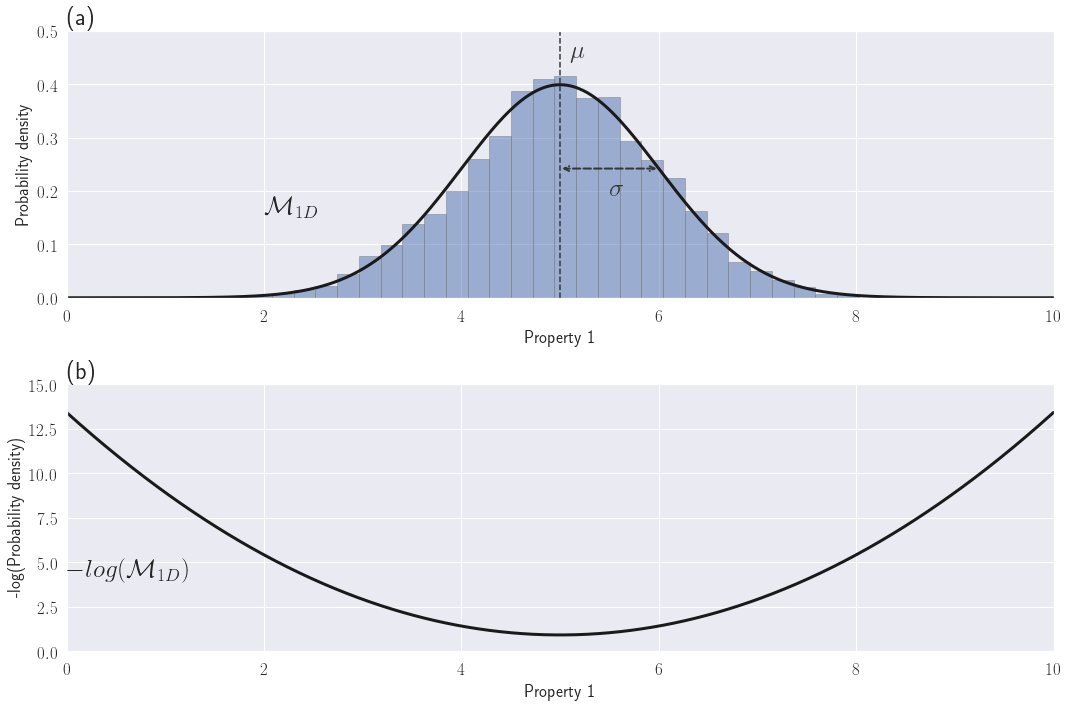
\includegraphics[width=\columnwidth]{./Fig/LowRes/Gaussian_to_Quadratic_1C.png}
\caption{(a) Examples of a Gaussian distribution in 1D for one physical property and (b) its quadratic negative-log equivalent}
\label{GaussianQuadratic}
\end{figure}

\begin{figure}
\centering
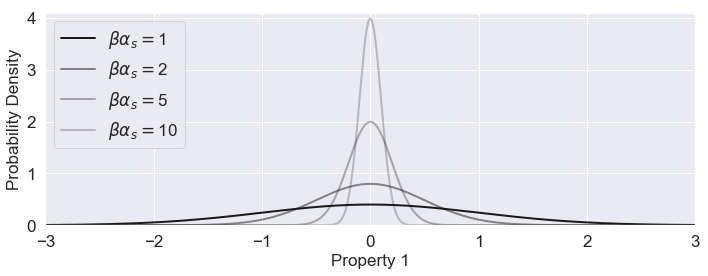
\includegraphics[width=\linewidth]{./Fig/LowRes/Gaussian1D_ConfidenceLevel.png}
\caption[]{Gaussian distributions for various confidence parameters}
\label{fig:ConfidenceLevel}
\end{figure}

Defining the smallness prior as a least-squares term such as in equation \ref{smallness_l2} thus assumes a Gaussian distribution of the model $\mathbf{m}$ values around the reference model. This is unlikely to correspond to the true physical property distribution, especially when the initial model is a half-space as commonly used. With the Tikhonov approach, the incorporation of knowledge about the physical properties can only be done locally at fixed locations defined by the users \citep{Lelievre2009}. A more versatile method is required.

Our focus is on designing a more meaningful and dynamically updatable prior for the smallness term $\mathcal{P}_{s}(\mathbf{m})$ when non-geophysical data are available but not necessarily well located. This will allow us to guide the model $\mathbf{m}$ towards producing an expected petrophysical distribution as well as capturing geological features. The inclusion of various types of information is done through the prior distribution. Our goal is thus to characterize each optimization process in Fig. \ref{graph_simple} as a MAP estimate. We have addressed the geophysical inversion problem (Fig. \ref{graph_simple}, process 1). We now focus on the petrophysical characterization and geological identification.


\subsection{Gaussian mixture model representation of petrophysical information} \label{PetrophysicsSection}

To include physical property information into the inversion, we first need to define a way to model the physical property distributions. Our choice is to use a Gaussian mixture model, where each geological unit's physical property is represented by a Gaussian distribution.

Consider that we are given a petrophysical dataset. We have $n$ samples, denoted $\{s_i,i=1..n\}$, which represent the measured physical properties. For each sample we know its current geological classification. This is denoted by $j=\left\{1..c\right\}$ where $c$ is the number of distinct geological units. We can use the geological classification as a categorical variable. A sample $i$ belonging to unit $j$ is noted $s_{i\in j}$.

\begin{figure}
\centering
\includegraphics[width=\columnwidth]{./Fig/LowRes/GaussianMixture_1D.png}
\caption{Examples of a Gaussian mixture like samples sets. (a) A GMM with two distinct units (the approximation in equation \ref{smallness_petro} is valid). (b) A GMM with overlapping units, the approximation in equation \ref{smallness_petro} is not valid.}
\label{GaussianMixture}
\end{figure}

For each geological unit $j$, we can fit a Gaussian probability density distribution. If the unit does not follow a Gaussian distribution, we can often project the physical properties into a transformed space where it appears approximately Gaussian, such as a log-space for electrical conductivity or magnetic susceptibility (see the notion of mapping in the SimPEG framework as defined in \cite{Cockett2015,SeogiMapping}). With known labels, the MLE of the Gaussian distribution parameters for each unit $j=\{1..c\}$, its mean $\mu_j$ and its variance $\sigma_j^2$ (or standard-deviation $\sigma_j$), plus its proportion $\pi_j$ among the dataset, are given in equations \ref{MLE-weights} to \ref{MLE-cov}:

\begin{align}
\pi_j &= \frac{n_j}{n}
\label{MLE-weights}
\end{align}

\begin{align}
{\mu}_j &= \frac{1}{n_j}\sum_{i=1}^{n_j}{s}_{i \in j}
\label{MLE-means}
\end{align}

\begin{align}
\sigma_j^2 & = \frac{1}{n_j}\sum_{i=1}^{n_j}({s}_{i \in j}-{\mu}_j)^2
\label{MLE-cov}
\end{align}

where the ${s}_{i \in j}$ are our $n_j$ physical property measurements for each geological unit $j$.

The full probability function to observe an unlabeled physical property data point ${s}_i$ can be written as a Gaussian mixture model (GMM) (see also Figs \ref{GaussianMixture}a and b):

\begin{align}
&\mathcal{P}({s}_i|\Theta) = \sum_{j=1}^c \pi_j \mathcal{N}({s}_i|{\mu}_j,\sigma_j^2) \label{GMM}
\end{align}

The variable $\Theta$ holds the GMM global variables $\Theta= \left\{\pi_j, {\mu}_j, \sigma_j^2\right\}_{j=1..c}$. A GMM is a parametric probability density distribution that can fit any continuous probability density distribution, when its number of clusters tends to infinity \citep{Murphy:2012:MLP:2380985}. It has gained popularity in recent years for representing geological and petrophysical information \citep{Giraud2017, Grana2010, Grana2017,Granek_2011}.

We denote $\mathbf{z}$ as our categorical variable for the labels, i.e. our geological classification. We call this variable our membership. Given an unlabeled data point ${s}_0$, its membership $z_0$ takes the value of the geological unit with the highest probability (see equation \ref{MAP_z_physProp}).

\begin{equation}
&z_0 = \mathop{\hbox{argmax}}\limits_{z \in \left\{1..j\right\}}\mathcal{P}(s_0|z)\mathcal{P}(z) \label{MAP_z_physProp}
\end{equation}
with:
\begin{equation}
&\mathcal{P}(z) = \pi_z \text{ and}\label{weight_z_prior}
\end{equation}
\begin{equation}
&\mathcal{P}(s_0|z)=\mathcal{N}({s}_0| {\mu}_{z},\sigma_{z}^2)
\end{equation}

Note that equation \ref{MAP_z_physProp} defines a MAP estimate of the geological identifier $\mathbf{z}$. The parameters $\left\{\pi_j\right\}_{j=1..c}$ represent our prior expectation of observing a certain unit before observing ${s}_0$ (equation \ref{weight_z_prior}). This MAP estimate will be our template for designing the geological identification process in our framework (Fig. \ref{graph_simple}, process 3).

The only posterior distribution left to define is for the petrophysical characterization process. We wish to determine MAP estimates of the GMM parameters when labels are unknown (Fig. \ref{graph_simple}, process 2). This is done in section \ref{UpdateTheta}.

%%%%%%%%%%%%%%%%%%%%%%%%%%%%%%%%%%%%%%%%%%%%%%%%%%%%%%%%%%%%%%%%%%%%%%%%%%%%%%%
\section{Gaussian mixture model as smallness prior for geophysical inversion} \label{section:Framework}


\subsection{Gaussian mixture model prior definition} \label{section:GMMprior}

Suppose we are given petrophysical and geological information about the geophysical model that we want to recover. Petrophysical information can include mean or variance values of physical properties for different geological units. Geological information can consist of an expected number of distinct units or an anticipation of encountering certain rock units in particular locations. We need to design a prior that offers the maximum flexibility for representing that petrophysical and geological prior knowledge.

In equation \ref{mixturemodel} we propose a GMM that is designed to serve as a prior on $\mathbf{m}$, whose parameters are both spatially (index $i$) and lithologically (index $j$) dependent. Our probability function is:

\begin{equation}
\mathcal{M}(\mathbf{m}|\Theta) = \prod_{i=1}^n \sum_{j=1}^c \mathcal{P}(z_{i}=j)\mathcal{N}({m}_i|{\mu}_j, {w}_{i}^{-2}\sigma_j^2)
\label{mixturemodel}
\end{equation}

where:
\begin{itemize}
\item $c$ is the number of distinct rock units, or clusters.
\item $n$ is the number of active cells in the mesh.
\item ${m}_i$ represents our physical property value at the $i^{\text{th}}$ cell.
\item $\mathbf{z}$ describes the membership to a certain rock unit.
\item $\mathcal{P}(z_{i}=j)$ represents our geological information. It is the prior probability of observing rock unit $j$ at location $i$ (vector notation: $\mathcal{P}(\mathbf{z})$). It can be either constant over the whole area, then representing an expected relative volume of each unit denoted by the global proportion $\pi_j$, or locally set if the information is available (e.g borehole logs, outcrops or geological modeling (see \cite{Giraud2017})).
\item ${\mu}_j$ is the mean physical property of rock unit $j$.
\item ${w}_{i}^{-2}\sigma_j^2$ is the variance of the rock unit $j$ at the $i^{\text{th}}$ cell. It includes both the expected physical property variance $\sigma_j^2$ of the rock unit $j$ globally and a local prior confidence ${w}_{i}^2$ that, at a certain cell $i$, the model value ${m}_i$ should belong closer or farther away from the mean ${\mu}_j$ of the rock unit $j$. Those $\mathbf{w}$ weights can be used to include depth or sensitivity weighting.
\item $\Theta$ holds the GMM global variables $\Theta= \left\{\pi_j, {\mu}_j, \sigma_j^2\right\}_{j=1..c}$.
\end{itemize}

Instead of adding an extra term in the objective function, we use the previously defined GMM probability distribution (equation \ref{mixturemodel}), representing our current geological and petrophysical knowledge, as our smallness prior. To have consistency with the Tikhonov framework, such as that defined in equation \ref{gaussian_prior}, we write:

\begin{equation}
\mathcal{P}_{s}(\mathbf{m}) \propto \mathcal{M}(\mathbf{m}|\Theta)^{\beta\alpha_s} \label{mixture_prior}
\end{equation}

To formulate our objective function, we apply a negative logarithm to the new posterior distribution, which uses the GMM probability distribution as the smallness prior (equation \ref{mixture_prior}). The resulting smallness term is then:

\begin{equation}
\Phi_s(\mathbf{m}) = - \sum_{i=1}^{n} \log\left(\sum_{j=1}^c \mathcal{P}(z_i=j) \mathcal{N}({m}_i|{\mu}_j, {w}_{i}^{-2}\sigma_j^2)\right) \label{full_smallness}
\end{equation}

Although we have had positive results with using the above \textit{LogSumExp} function in the smallness regularizer (the exponential function being in the Gaussian distribution $\mathcal{N}$), there are benefits of using the following approximation. Gaussian distributions decay exponentially. If the units have distinguishable enough contrasts, it is reasonable to approximate the \textit{LogSumExp} function in equation \ref{full_smallness} by its locally dominant quadratic term. This means considering only the most probable rock unit for each cell given the current model $\mathbf{m}$. The other terms of the summation are deemed negligible. For example consider the 1D physical property distributions in Fig. \ref{GaussianMixture}. For the physical property distribution in Fig. \ref{GaussianMixture}(a), the individual Gaussian functions representing each rock unit can locally approximate the GMM extremely well. On the other hand, for the physical property distribution displayed in Fig. \ref{GaussianMixture}(b), there is too much overlap between the two individual Gaussian components. Individually they are not a good approximation to the full GMM distribution and the above assumption is incorrect. In that case, one can either work with the full expression shown in equation \ref{full_smallness}, or potentially re-evaluate whether the individual distributions are distinct enough to be considered as separate units. As a rule of thumb, contrasts are deemed distinguishable enough to apply this approximation if the centers of two clusters are separated by at least three times the largest standard deviation. By using the parameters of the most likely cluster at each active cell we can approximate $\Phi_{s}(\mathbf{m})$ as:

\begin{equation}
&\Phi_{s}(\mathbf{m}) = \frac{1}{2}||W_{s}(\Theta, \mathbf{z}^*)(\mathbf{m}-\mathbf{m}_{\text{ref}}(\Theta, \mathbf{z}^*))||_2^2 \label{smallness_petro}
\end{equation}
with:
\begin{equation}
&\mathbf{z^*} = \mathop{\hbox{argmax}}\limits_{\mathbf{z}}\mathcal{P}(\mathbf{m}|\mathbf{z})\mathcal{P}(\mathbf{z}) \label{membership}
\end{equation}
\begin{equation}
&\mathbf{m}_{\text{ref}}(\Theta, \mathbf{z}^*) = {\mu}_{\mathbf{z}^*} \label{mref_update}
\end{equation}
\begin{equation}
&W_{s}(\Theta, \mathbf{z}^*) = \text{diag}({\mathbf{w}}\circ{\sigma_{\mathbf{z}^*}^{-1}}) \label{Ws_update}
\end{equation}

Note the similarity of the smallness term in equation \ref{smallness_petro} with the Tikhonov formulation (equation \ref{smallness_l2}). This allows us to generate a petrophysically and geologically guided inversion that uses traditional algorithms, and thus can rely on the research literature on the Tikhonov approach.

Our approach, regarding the regularized geophysical problem, can be summarized as follows: At each iteration, we first identify the most probable unit for each cell; we call it its membership, and store it in the categorical vector $\mathbf{z}$ (equation \ref{membership}). The reference model $\mathbf{m}_{\text{ref}}$ and smallness weights $W_s$ are then updated according to the membership $\mathbf{z}$. The reference model at each cell takes the physical property mean value of the most likely unit ${z^*_i}$ (equation \ref{mref_update}). The smallness weights depend on the value of the corresponding variances and on our local weights (e.g depth or sensitivity weighting; see equation \ref{Ws_update}). These updates represent the newly acquired knowledge on $\mathbf{m}$ according to the petrophysical distribution $\Theta$ and the geological information $\mathcal{P}(\mathbf{z})$. We refer to the updated reference model as the learned reference model. The next inversion step then pushes each cell of the mesh towards the mean of its most probable rock unit. The strength of the push is proportional to the variance of the physical property for that unit (the higher the variance, the less we push), and our weights $\mathbf{w}$.

Equations \ref{membership} defines the MAP process for the geological identification (Fig. \ref{graph_simple}, process 3). Equations \ref{mref_update} and \ref{Ws_update} link the petrophysical and geological information with the geophysical inversion.

One could proceed by using the means and variances fitted on the petrophysical data, as well as the proportions from the geological data, to compute $\mathbf{z}$, $\mathbf{m}_{\text{ref}}$ and $W_s$ at each iteration (equation \ref{membership}, \ref{mref_update} and \ref{Ws_update}). However when this knowledge is incomplete or uncertain, our estimated GMM may not be accurate. \cite{McAuslan2015} have investigated that issue and shown that inaccurate petrophysical information can significantly affect the recovered model. \cite{Sun2015, Sun2016, Sun2017} partially overcome this by updating the cluster centers through the iteration process; they average the observed means in the geophysical model with the means from the petrophysical measurements through a separate clustering optimization problem. We generalize this approach to all of the parameters of the GMM. In the next section \ref{UpdateTheta}, we formulate the petrophysical characterization step of our framework (Fig. \ref{graph_simple}, process 2) as a MAP estimation process.


\subsection{Updating the Gaussian mixture model} \label{UpdateTheta}

One can either consider that the GMM parameters derived from petrophysical and geological data give the best estimation of the true distribution, or that it is only an approximation, and additional information can be obtained from the geophysical model during the inversion \citep{Sun2015}. We prefer this later approach. Since the prior knowledge might be incomplete or only known qualitatively, it is important to mitigate possible biases that can affect the final recovered model \citep{McAuslan2015}. For that purpose \citeauthor{Sun2015} updated each cluster center of their fuzzy C-means clusters through a weighted average of the expected center from the petrophysical data with the observed center in the geophysical model. From a statistical view point, this resembles the use of a MAP estimator to find the cluster means applied to the geophysical model itself, with the addition of a conjugate prior based on the petrophysical data. The notion of conjugate prior was first introduced in \cite{conjugateprior}. By definition, a prior is called a conjugate prior to the likelihood function if the posterior belongs to the same family of probability distributions as the prior. For example the Gaussian distribution is self-conjugate. This means that if the likelihood follows a Gaussian distribution, choosing a Gaussian prior ensures that the posterior also belongs to the same family of probability density distributions. We use the conjugate prior approach to formalize the update of the means done in \cite{Sun2015} and generalize it to the other GMM parameters.

Obtaining the GMM parameters $\Theta$ is thus made part of the iterative inversion process. We define the petrophysical characterization process (Fig. \ref{graph_simple}, step 2) as a MAP estimator for $\Theta$. This MAP estimate benefits both from the petrophysical and geological data known prior to the inversion and the current geophysical model. After each geophysical inversion iteration, and before updating the membership $\mathbf{z}$, we learn the mixture parameters $\Theta$ using the current geophysical model $\mathbf{m}$ and our confidence in the prior knowledge $\Theta_{\text{prior}}$. We define a posterior distribution on $\Theta$, given the geophysical model $\mathbf{m}$ and prior knowledge, as:

\begin{equation}
\mathcal{P}(\Theta|\mathbf{m}) \propto \mathcal{M}(\mathbf{m}|\Theta)\mathcal{P}(\Theta)
\label{theta_posterior}
\end{equation}

In section \ref{PetrophysicsSection}, the problem of fitting a single Gaussian distribution to each unit, and thus defining its petrophysical mean and variance, was made easy by knowing the geological unit of each sample. A much harder problem is to recover the full multimodal probability function described in equation \ref{GMM} when there are missing labels. For example, in an inverted geophysical model $\mathbf{m}$, most locations for the geological units are unknown except where we have drillholes and outcrops. In fact, this is usually the information we are trying to determine. The categorical variable $\mathbf{z}$ that represents our geological classification is now a hidden variable that we want to find along with the GMM parameters. Clustering algorithms are especially designed for this sort of task. The Expectation Maximization (EM) Algorithm \citep{MR0501537} is one of the most widely used algorithms for semi-supervised and unsupervised learning in mixture modelling. It allows us to fit the parameters $\Theta=\left\{\pi_j, {\mu}_j, \sigma_j^2\right\}_{j=1..c}$ of a mixture model to a multimodal distribution with partial or no labeling. The EM algorithm in its original form is a MLE, thus no prior information is involved. To include prior information in the algorithm, and thus find a MAP estimate for the posterior distribution on $\Theta$ shown in equation \ref{theta_posterior}, we use a MAP variation of the Expectation-Maximization algorithm (also introduced in \cite{MR0501537}); we refer to this algorithm as the MAP-EM algorithm.

For the MAP-EM algorithm, we need to choose how to model the prior $\mathcal{P}(\Theta)$ for each type of parameter. We can follow either a conjugate prior or semi-conjugate prior approach as described by \cite{Murphy:2012:MLP:2380985}. Each step of the MAP-EM algorithm applied to a GMM with a conjugate or semi-conjugate prior can be understood as a weighted average of the observed parameters with their priors. Figure \ref{example_MAPEM} shows an example of such a MAP estimate of the GMM parameters. We define the input of each prior function so that an input value of unity denotes an equal weighting of the observed and prior distributions. We refer to those input values as our confidences in the GMM prior parameters. Confidences of zero in the prior generate a MLE estimator; the prior parameters are not taken into account and the algorithm reverts to the normal EM algorithm. Infinite confidences in the prior fix the GMM's parameters equal to their priors value.

\begin{figure}
    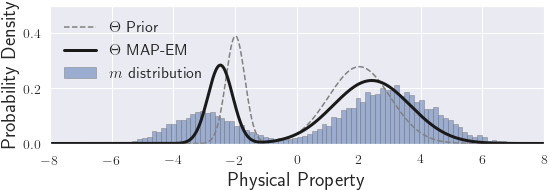
\includegraphics[width=\columnwidth]{./Fig/LowRes/example_MAPEM.png}
    \caption{Illustration of fitting a Gaussian mixture model with parameters $\Theta$ through the MAP-EM algorithm, given the geophysical model $\mathbf{m}$ and the prior petrophysical distribution $\Theta_{\text{prior}}$ with all confidences set to unity}
    \label{example_MAPEM}
\end{figure}

The MAP-EM algorithm is an iterative process. We initialize by starting with the parameters determined at the previous cycle. The usual stopping criteria defined in the literature for the MAP-EM algorithm is to define a minimum increase of the posterior probability density value. At each MAP-EM iteration $(k)$, we first compute the responsibility $\left\{n_{ij}\right\}_{j=1..c,i=1..n}$ of each cluster $j$ for each point ${m}_i$. This is referred as the E-step in the EM algorithm and it stays unchanged in its MAP-EM variation:

\begin{equation}
n_{ij}^{(k)} = \frac{\mathcal{P}(z_i=j)^{(k-1)}\mathcal{N}({m}_i|{\mu_j}^{(k-1)}, ({\sigma_j^2})^{(k-1)})}{ \sum_{t=1}^c \mathcal{P}(z_i=t)^{(k-1)} \mathcal{N}({m}_i|{\mu_t}^{(k-1)}, ({\sigma_j^2})^{(k-1)})} \label{responsibilities}
\end{equation}

We then compute the MAP-EM steps at iteration $(k)$ with respect to the global proportion weights $\left\{\pi_j\right\}_{j=1..c}$, means $\left\{\mu_j\right\}_{j=1..c}$ and variances $\left\{\sigma_j^2\right\}_{j=1..c}$ of the GMM. These steps are referred to as the M-step in the EM-algorithm. The MAP-EM variation M-step includes prior information as part of the iterative update.

The global proportion weights follow a categorical distribution whose conjugate prior is the Dirichlet distribution (equation \ref{pi_prior}):

\begin{equation}
\mathcal{P}(\mathbf{\pi}) = \text{Dir}({\zeta}\pi_{prior}V-1) \label{pi_prior}
\end{equation}

At iteration $(k)$, the resulting posterior estimate of $\left\{\pi_j\right\}_{j=1..c}$, given $\left\{{\pi_j}_{prior}\right\}_{j=1..c}$ and with confidence $\left\{\zeta_j\right\}_{j=1..c}$, is shown in equation \ref{pi_update}:

\begin{align}
&\pi^{(k)}_j = \frac{V_{j}^{(k)}+\zeta_j {\pi_j}_{prior}V}{V(1+\sum_{t=1}^c \zeta_t {\pi_t}_{prior})} \label{pi_update}
\end{align}
with:
\begin{align}
&V_{j}^{(k)} = \sum^n_{i=1} v_i n_{ij}^{(k)} \label{VolumeProportions}
\end{align}
and
\begin{align}
V=\sum^n_{i=1} v_i
\end{align}

where $v_i$ is the volume of the $i^\text{th}$ cell and $V$ is the volume of the active mesh. The addition of these volume weights is necessary because the cells of our mesh can have different sizes. We want to use a prior information that is mesh-independent. That is why we use volumetric proportions instead of cell counts, which is the way the EM algorithm is usually implemented.

The full conjugate priors of the likelihood function in equation \ref{theta_posterior} for the means and variances are not independent of each other and they follow a Normal-Inverse-Gamma distribution \citep{Murphy:2012:MLP:2380985}. However using the full conjugate prior approach for the variances can be harmful in the first few iterations. Mean values from models at early iterations may be far from their final target values and that would drive the GMM estimated by MAP-EM to have very high variances (to compensate for the difference between the observed and prior means) and thus compromise the clustering (see Appendix \ref{appendix:full_conjugate} for further details).

To avoid this issue, a semi-conjugate prior approach is possible where the dependency of the means and variances is avoided by using the conditional distributions as priors. In this case the semi-conjugate prior for the means follows a Gaussian distribution (equation \ref{mu_semiprior}) while the semi-conjugate prior for the variances follows an Inverse-Gamma distribution (equation \ref{sigma_semiprior}). As usually done in the statistics literature \citep{Murphy:2012:MLP:2380985}, we use an alternative parameterization of the Inverse-Gamma distribution called the Inverse Chi-Squared distribution. This re-parameterization allows for a simpler definition of the parameters. The semi-conjugate priors for the means and variances, with respective confidences $\{\kappa\}$ and $\{\nu\}$, are:

\begin{align}
&\mathcal{P}({\mu}| \sigma^2) = \mathcal{N}({\mu}|{\mu}_{prior}, ({\kappa}\pi_{prior}V)^{-1}) \label{mu_semiprior} \\
\end{align}
and:
\begin{align}
&\mathcal{P}(\sigma^2|{\mu}) = \mathcal{X}^{-2}(\sigma^2|{\nu}{\pi}_{prior}V,\sigma_{prior}^2) \label{sigma_semiprior}
\end{align}

Note that if we put prior information only on the means, or only on the variances, then this is a full conjugate prior. The semi-conjugate prior approach arises only when we put prior information on both means and variances (meaning that $\{\kappa\}$ and $\{\nu\}$ are both non zero).

The update of the means is the same for both the full conjugate and semi-conjugate prior approaches. The current $(k)$ posterior estimate of the means $\left\{{\mu}_j\right\}_{j=1..c}$ is a weighted average of the MLE estimates $\left\{\bar{\mathbf{m}}_j\right\}_{j=1..c}$ from equation \ref{MLE-means}, using the geophysical model as the samples, with the prior means $\left\{{{\mu}_j}_{prior}\right\}_{j=1..c}$ and with confidences $\left\{\kappa_j\right\}_{j=1..c}$. This update to the means is shown in equation \ref{mu_update}:

\begin{align}
&{\mu}^{(k)}_j=\frac{V_{j}^{(k)}{\bar{{m}}}_j^{(k)} + \kappa_j {\pi_j}_{prior} V {{\mu}_j}_{prior}}{V_{j}^{(k)}+\kappa_j {\pi_j}_{prior} V} \label{mu_update}
\end{align}
with:
\begin{align}
&{\bar{{m}}}_j^{(k)} = \frac{\sum^n_{i=1} v_i n_{ij}^{(k)} {m}_i}{V_{j}^{(k)}}
\end{align}


For the semi-conjugate prior, the current $(k)$ posterior estimate of the variances $\left\{{\sigma_j^2}\right\}_{j=1..c}$, given in equation \ref{sig_update}, is a weighted average, with confidence $\left\{\mathbf{\nu}_j\right\}_{j=1..c}$, of the MLE estimations of the variances $\left\{{\sigma^2_{\bar{\mathbf{m}}}}_j\right\}_{j=1..c}$ from equation \ref{MLE-cov} with their prior $\left\{{\sigma_j^2}_{prior}\right\}_{j=1..c}$.

\begin{align}
&{\sigma_j^2}^{(k)} = \frac{{{V_{j}^{(k)}} {\sigma^2_{\bar{\mathbf{m}}}}_j}^{(k)} + \nu_j {\pi_j}_{prior} V {\sigma_j^2}_{prior}}
{{V_{j}^{(k)}} + \nu_j {\pi_j}_{prior} V} \label{sig_update}
\end{align}
with:
\begin{align}
&{\sigma^2_{\bar{\mathbf{m}}}}_j^{(k)} =\frac{1}{{V_{j}^{(k)}}} \sum_{i=1}^{n} v_i n_{ij}^{(k)}({m}_i-\bar{{m}_j}^{(k)})^2
\end{align}

We run fully the MAP-EM algorithm to learn a new petrophysical distribution with parameters $\Theta = \left\{\pi_j, \mathbf{\mu}_j, \sigma_j^2\right\}_{j=1..c}$ after each iteration $(t)$ of the geophysical inversion process, using the current geophysical model $\mathbf{m}^{(t)}$ and the prior petrophysical distribution $\Theta_{\text{prior}}$.

This completes our derivation. Equation \ref{theta_posterior} in particular describes the MAP estimator for the petrophysical characterization. Our three MAP estimates are interconnected through the sharing of the geophysical model, petrophysical distribution and geological classification. The final framework is summarized in Fig. \ref{graph_math}, which is the completed version of the previous diagram (Fig. \ref{graph_simple}). The next step is to numerically implement this procedure. That is done in the following section.

\begin{figure}
    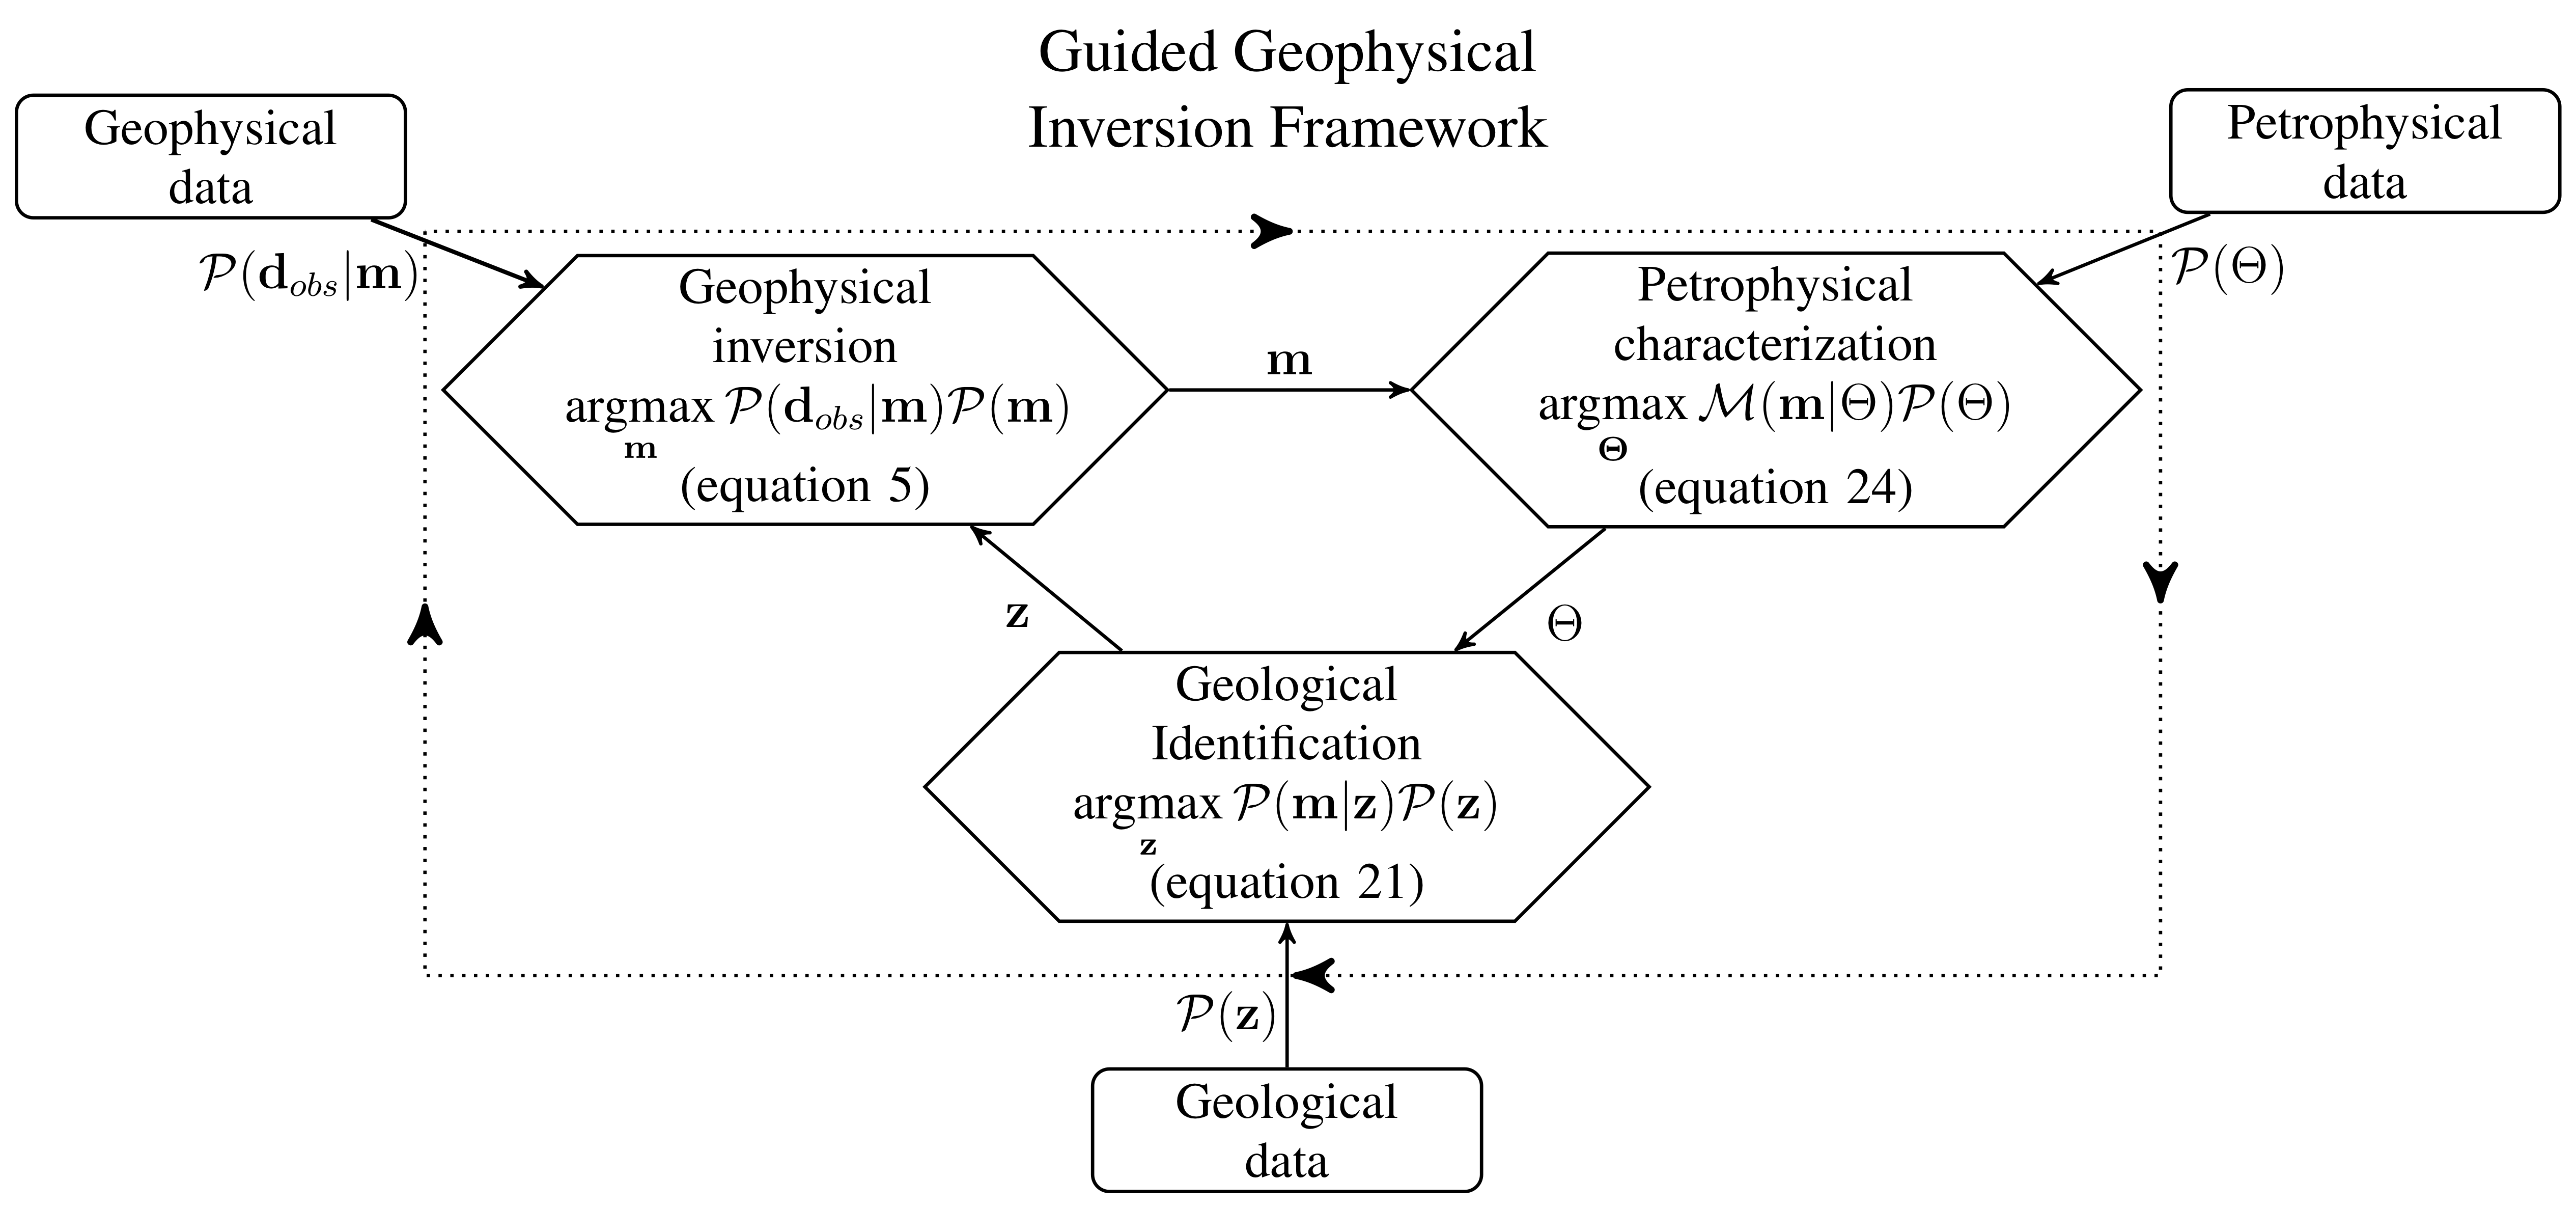
\includegraphics[width=\columnwidth]{./Fig/LowRes/Framework_with_equationsnumbers.png}
    \caption{A graph approach illustrating how the various posterior distribution MAP estimate processes are interlocked with each other.}
    \label{graph_math}
\end{figure}

%%%%%%%%%%%%%%%%%%%%%%%%%%%%%%%%%%%%%%%%%%%%%%%%%%%%%%%%%%%%%%%%%%%%%%%%%%%%%%%
\section{Numerical Implementation} \label{section:Implementation}

Our framework defines three inverse problems that are interconnected and special care is required to ensure that each is reasonably well solved. In this section we look at some of the essential implementation elements of this framework. A comprehensive algorithm and a flowchart can be found in appendix \ref{section:pseudocode}. However, before going into the details of the pseudocode, we formalize the concept of fitting the petrophysical and geological data and thus define a stopping criteria for our numerical solution.


\subsection{Petrophysical target misfit and inversion stopping criteria} \label{section:stopping}

The smallness term, such as defined in equation \ref{smallness_petro}, measures how well the geophysical model fits the petrophysical and geological data through the GMM. We need to define a target for this misfit term.

For the definition and evaluation of the petrophysical target misfit, we  focus on the petrophysical and geological information contained in the smallness term that is summarized in equations \ref{smallness_petro_2} to \ref{Ws_update_2} and identified as $\Phi_{petro}$.

\begin{align}
&\Phi_{petro}(\mathbf{m}) = \frac{1}{2}||W_{s}(\Theta, \mathbf{z}^*)(\mathbf{m}-\mathbf{m}_{\text{ref}}(\Theta, \mathbf{z}^*))||_2^2 \label{smallness_petro_2}
\end{align}
with:
\begin{align}
&\mathbf{z^*} = \mathop{\hbox{argmax}}\limits_{\mathbf{z}}\mathcal{P}(\mathbf{m}|\mathbf{z})\mathcal{P}(\mathbf{z}) \label{membership_2} \\
\end{align}
\begin{align}
&\mathbf{m}_{\text{ref}}(\Theta, \mathbf{z}^*) = {\mu}_{\mathbf{z}^*} \label{mref_update_2}
\end{align}
\begin{align}
&W_{s}(\Theta, \mathbf{z}^*) = \text{diag}({\sigma_{\mathbf{z}^*}^{-1}}) \label{Ws_update_2}
\end{align}

At each iteration, the $i^{\text{th}}$ element $(m_i-{m_{\text{ref}}}_i)$ is a Gaussian random variable of mean zero and variance $\sigma_i^2$. Consequently elements in $W_s(\mathbf{m}-\mathbf{m}_{\text{ref}})$ are Gaussian with zero mean and unit standard deviation. Thus $\Phi_{petro}$ is a chi-squared statistical parameter with expectation:

\begin{align}
\text{E}\lbrack\Phi_{petro}\rbrack &= \Phi_{petro}^* = \frac{n}{2} \label{petrotargetmisfit}
\end{align}

This defines the petrophysical target misfit value $\Phi_{petro}^*$ for $\Phi_{petro}$ as being half the number of active cells $n$ in the geophysical model (equation \ref{petrotargetmisfit}). As one condition for stopping our algorithm we want to find an $\mathbf{m}$ for which $\Phi_{petro}$ is less than or equal to $\Phi_{petro}^*$.

The equation \ref{smallness_petro_2} for evaluating the petrophysical stopping criterion omits the weights $\mathbf{w}$ (equation \ref{smallness_petro}). The additional weights $\mathbf{w}$ are used to include depth or sensitivity weighting, which are more related to the physics of the survey rather than to the desired properties of the geophysical model. We have taken two approaches; the first is to minimize $\Phi_s$ but keep the stopping criterion attached to $\Phi_{petro}$. The second is to minimize and measure the stopping criterion using $\Phi_s$ after adjusting the target misfit value to be $||\mathbf{w}||^2_2/2$. Thus far we prefer the former approach because the second has lead us in certain cases to underfit the petrophysical distribution. The examples, developed in sections \ref{section:synthetic_examples}, all use various weighting strategies and the $\Phi_{petro}$ stopping criterion approach.

We note this stopping criterion for the petrophysical data is analogous to the geophysical data misfit criterion. The geophysical data misfit term, such as defined in equation \ref{datamisfit}, is also a sum of Gaussian variables with zero mean and unit standard deviation. Thus a reasonable target misfit, such as introduced in \cite{Parker}, is:

\begin{align}
& {\Phi_d^*} = \frac{n_\text{d}}{2}
\label{geophytargetmisfit}
\end{align}

where $n_\text{d}$ is the number of geophysical data.

Our algorithm stops when we have found a model that simultaneously has both $\Phi_d$ and $\Phi_{petro}$ equal or below their respective target value $\Phi_d^*$ and $\Phi_{petro}^*$. Reaching multiple target misfits adds a new challenge to solving the inverse problem. We address this in the following section as we work through the important components of the pseudocode.


\subsection{Pseudocode and Weighting strategies} \label{weighting}

At each iteration of our PGI algorithm, three inverse problems need to be solved. Our algorithm is provided in two forms in appendix \ref{section:pseudocode}. The first is a pseudocode (algorithm \ref{algo:algorithm}), the second is a detailed flowchart that is linked to the pseudocode (Fig. \ref{Flowchart}). Here we discuss some of the important elements that assist in understanding the details of the algorithm.


\subsubsection{Step 1: Initialization}

We are solving three MAP problems. Each needs to be initialized with an initial geophysical model $\mathbf{m}_0$, a petrophysical distribution $\Theta_0$ and  a membership $\mathbf{z}_0$ respectively. We usually have these elements consistent with each other. For example, the initial reference model is usually the starting model. We can start from a background half-space $\mathbf{m}_0$, whose value is the same as in $\Theta_0$, and set $\mathbf{z}_0$ at the background unit everywhere.

For the success of a geophysical inversion, the choice of the various weighting parameters can be critical. Our framework still uses a conventional geophysical inversion objective function, and hence previous studies and good practices are still applicable. We need to provide uncertainties $W_d$ for the geophysical data least-squares misfit term (equation \ref{datamisfit}). The objective function (equation \ref{tikhonov}) requires a reference model and initial weighting parameters. A common practice is to start with a large $\beta$ and then decrease its value during the inversion iterative process \citep{betachoice2004}. For the smallness and derivative weights $\left\{ \alpha \right\}$, the similarity of our formulation with the Tikhonov approach allows us to rely on the existing literature (e.g \cite{Lelievre2009,doi:10.1190/1.9781560801719.ch5,Williams_2008}).

For the petrophysical inverse problem, we initialize the petrophysical distribution by setting $\Theta^0=\Theta_{\text{prior}}$. We thus need to design $\Theta_{\text{prior}}$. For each unit, when petrophysical measurements or a priori estimates are available, both the mean and variance of the GMM cluster can be set. When no information is available, it is still required to provide some estimate for the variances. These prior variances can be thought of as petrophysical noise levels, analogous to the geophysical noise levels. They play an essential role in determining the petrophysical target misfit and regulate the clustering of each unit around its, to be determined, mean value. The proportions represent geological knowledge. When they are set globally, they represent the expected relative volume of each unit. The choice of confidences in the prior parameters is still a challenging question (see section \ref{UpdateTheta} for definitions). When the petrophysical information is well-known, values of unity, or higher, have worked well. When no petrophysical information is known a priori, values of unity or above for the confidences in the prior variances are used, while confidences in the means and proportions are set to zero. In the examples section (section \ref{section:synthetic_examples}) we show examples for both the known and unknown petrophysical information cases.

The starting geological model can be determined by the starting geophysical model and petrophysical distribution. Additional local knowledge about the geology can be added through the choice of local proportion values for the GMM. We show a simple demonstration through the 2D resistivity example (section \ref{DCexample}). For example, knowing that a unit appears at a certain location, can be added to the inversion. For that purpose we can locally set the proportion for this unit to unity, consequently giving a probability of zero for the other units at that same location.

This initialization completes step 1 in our pseudocode (algorithm \ref{algo:algorithm}) and flowchart (Fig. \ref{Flowchart}). The next step is to evaluate our stopping criteria and update the models.


\subsubsection{Step 2 - 5: Check convergence and update the model}

At step 2, we check if the convergence criteria $\Phi_d\leq\Phi_d^*$, and $\Phi_{petro}\leq\Phi_{petro}^*$ have been met. If these are not satisfied, then a model update is required. We start by taking a single Gauss-Newton step on the geophysical objective function \citep{NoceWrig06} (step 3).  Step 4 consists in running  the MAP-EM algorithm described in section \ref{UpdateTheta} to learn a new petrophysical distribution parameters $\Theta^{(t)}$, using the updated geophysical model $\mathbf{m}^{(t)}$. Finally at step 5 we update the membership $\mathbf{z}^{(t)}$, using $\mathbf{m}^{(t)}$ and $\Theta^{(t)}$ according to equation \ref{membership}. This updates the smallness weights and reference model for the next iteration, such as described in equation \ref{mref_update} and \ref{Ws_update}.


\subsubsection{Step 6: Updating $\beta$ and $\alpha_s$}

In this step we adjust our weights so that the inversion arrives at a solution that acceptably fits both the geophysical data and the GMM containing the geological and petrophysical data. We have two adjustable parameters, $\beta$ and $\alpha_s$. The parameter $\beta$ balances the data misfit with the total regularization function, while $\alpha_s$ allows us to adjust the importance of the smallness term.

Our current procedure uses a computationally inexpensive heuristic approach to find suitable $\beta$ and $\alpha_s$ parameters such that both geophysical and petrophysical misfits are equal or below their respective target value. We initially set $\beta$, and $\{\alpha\}$ to values we would use for a standard inversion. We first invoke a $\beta$-cooling to get towards a solution that fits the geophysical data. Once reached, we focus more on fitting the petrophysical data by adjusting $\alpha_s$.

If the geophysical data misfit term reaches a plateau before attaining its target, we decrease $\beta$ by a predetermined factor (step $6$, first case scenario). We think of $\beta$ as an outer-control parameter since it is a weighing for the entire regularization function, which includes smallness and gradient terms.

In our case we also want to find a solution that fits the petrophysical and geological data. For this we fine-tune the inner-control parameter $\alpha_s$. If the geophysical data misfit target $\Phi_d^*$ has been reached, but not the petrophysical data misfit $\Phi_{petro}^*$, we put more emphasis on the smallness model term. We increase $\alpha_s$ by a factor $\Phi_d^*/\Phi_d^{(t)}$ (step $6$, second case scenario). This is similar to the $\beta$-warming strategy described in \cite{Fournier2015}. Generally this allows us to focus the algorithm on reaching the petrophysical data misfit target without significantly altering the geophysical data misfit. If the geophysical data misfit is increased too much, then $\beta$ is reduced. In summary, we use $\alpha_s$ as a fine-tuning parameter as it is not adjusted until late stages of the inversion when the major structures have already been identified.

\subsubsection{Step 7: Final output}

The algorithm stops when both the geophysical and petrophysical misfits are below or equal to their respective targets. The PGI framework outputs three quantities: the recovered geophysical model, the learned petrophysical distribution and membership. The geophysical model fits both the geophysical data and the learned petrophysical distribution. The membership attributes a rock unit to each cell; we refer to this categorized model as a quasi-geological model, as proposed by \cite{QuasiGeologicalModel}.


\subsubsection{Options}

We have the possibility to include, or not, the learned reference model inside the smoothness components of the objective function. Our preferred strategy is to leave it out until we have reached the geophysical data misfit target and when only a small fraction of the membership $\mathbf{z}$ is changing. This avoids the creation of interfaces at locations that are likely to change later in the inversion. Once the learned reference model has stabilized we can then incorporate the reference model into the smoothness term. It promotes the creation of interfaces, which also help to reach the smallness target misfit if it has not yet happened. This strategy and its effects are illustrated in the DC example (section \ref{DCexample}).


\subsection{Convergence}

At each iteration, the gradient-step for the geophysical objective function is similar to that in the Tikhonov formulation. This step is guaranteed to be a descent direction for the objective function. The objective function to be minimized, however, changes because the solution of the MAP-EM problem changes the reference model and smallness weights. Fortunately the MAP-EM algorithm guarantees a decrease of the smallness term at each iteration. In other words the updated petrophysical distribution is guaranteed to be closer to the current geophysical model than the previous distribution.

Thanks to these properties, our algorithm usually reaches the geophysical target misfit at a rate comparable to the Tikhonov approach, and then requires only a few additional iterations to reach the petrophysical target misfit. Each PGI example presented in the next section \ref{section:synthetic_examples} runs in a number of iterations comparable to the Tikhonov inversion while reaching both of our stopping criteria. This is a significant result as this means applying this framework does not necessarily end in a massive loss of efficiency.

%%%%%%%%%%%%%%%%%%%%%%%%%%%%%%%%%%%%%%%%%%%%%%%%%%%%%%%%%%%%%%%%%%%%%%%%%%%%%%%
\section{Examples} \label{section:synthetic_examples}

In this section we present two synthetic examples and a field example that illuminate important aspects of our framework. These examples are available as part of the SimPEG package on Github at \url{https://github.com/simpeg-research/Astic-2019-PGI} \citep{PGIexamples}. Readers are invited to use the notebooks and reproduce the results.

The first example is a non-linear inverse problem in electromagnetics. Magnetotelluric data \citep{WardandHohmann} are acquired over a layered-earth that has sharp and smooth features. We are provided with the true petrophysical distribution and the goal is to use it, along with the MT data, to find a solution that has the desired features. We present the results at the various steps of the algorithm and display the updates done to the initial petrophysical and geological models that are used to guide the geophysical inversion.

In the second example, a DC resistivity profile \citep{WardandHohmann} is acquired over two cylinders. We demonstrate how this framework performs when the GMM is not known a priori. We also use this example to show how prior geological information can be included into the inversion.

The third example is an airborne Frequency-Domain Electromagnetics (FDEM) survey \citep{WardandHohmann} over a floodplain in Australia potentially contaminated by saline water. We highlight the influence of the choice of a reference model on the Tikhonov models. We then illustrate how the PGI approach can reduce ambiguity in the recovered features. This is achieved by constructing models in which the earth is assumed to have a certain number of distinct units. This sort of questions (what if there are $c$ units?), crucial for interpretation, are otherwise difficult to ask in a traditional Tikhonov setting.

\subsection{MT1D, layered and smooth Earth model: Demonstration of the framework}

In this example, we demonstrate how to use the PGI framework to include petrophysical information. We first highlight the gains made in the recovered geophysical model. We then provide details about how the PGI iterations proceed.

\begin{figure}
 \centering
 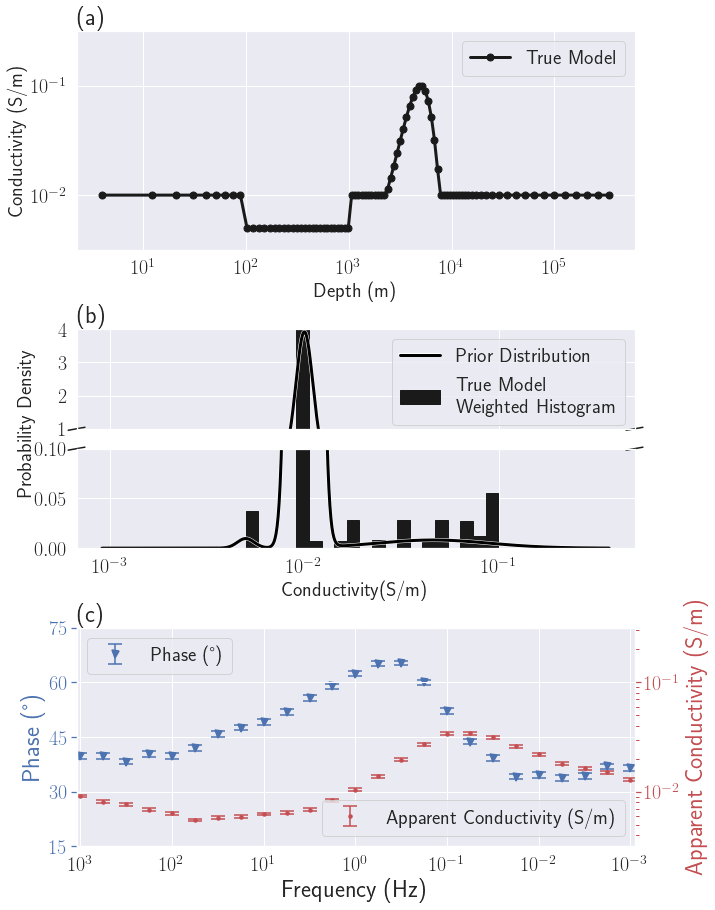
\includegraphics[width=\columnwidth]{./Fig/LowRes/MT1D_Setup.png}
 \caption[]{Setup of the MT1D example: (a) True geophysical model $\mathbf{m}_{\text{true}}$. The dots coincide with the cell centers in the discretized model. (b) True model weighted histogram and prior petrophysical distribution $\Theta_{\text{prior}}$; (c) MT data and uncertainties.}
 \label{Fig/LowRes/MT1D_Setup}
\end{figure}

\subsubsection{Setup}

For this example, inspired by \cite{tle-MT1D}, we want to recover a 1D earth model that is made up a resistive layer and a smoothly varying unit embedded in a uniform background. The conductivity model, which is discretized onto a mesh with $89$ cells, is shown in Fig. \ref{fig:MT1D_Setup}(a). The background unit has a conductivity of $0.01~\text{S/m}$ ($100~\Omega \text{m}$). The resistive unit ($5\cdot10^{-3}~\text{S/m}$ or $200~\Omega \text{m}$) is $900~\text{m}$ thick and starts at a depth of $100~\text{m}$. The smooth conductor, with a maximum conductivity of $0.1~\text{S/m}$ ($10~\Omega \text{m}$), is located between $2,300~\text{m}$ and $7,560~\text{m}$ depth. A log-scale, which is traditional for MT, is used.

In the MT experiment the electric and magnetic fields recorded at the earth’s surface are combined to generate impedances. In this example, data are collected at 25 logarithmically spaced frequencies between $10^{-3}$ and $10^3$ Hz. This generates 50 data composed of the real and imaginary components of the impedance for each frequency. Unbiased Gaussian noise with a standard-deviation of $2\%$ of the data value is added. We represent those observed data in the form of apparent conductivity and phase in Fig. \ref{fig:MT1D_Setup}(c).


\subsubsection{Initialization}

We first describe our initialization for both the Tikhonov and PGI algorithms. For the initial geophysical model $\mathbf{m}_0$, we choose a uniform half-space with the same conductivity as the background unit. For the PGI approach the starting membership $\mathbf{z}_0$ is set to the background unit everywhere. Both the Tikhonov and PGI approaches start with the same objective function; the models after the first iteration are thus identical. This helps for comparing results between the two approaches.

For the PGI approach we also need to provide a GMM to describe our prior petrophysical and geological information $\Theta_{\text{prior}}$. We use the exact information from the true earth model for the means and global proportions. For the variances, we use the true variance for the smooth unit. This unit is characterized by a wide distribution and thus it has a large variance. The background and the resistive unit are characterized by single values so their true variances are zero (Dirac distribution). We assign a standard deviation of $0.1~\ln(\text{S/m})$ (or variance of $0.01~[\ln(\text{S/m})]^2$) as an acceptable level of petrophysical noise for those two units. This prior petrophysical distribution can be visualized in Fig. \ref{fig:MT1D_Setup}(b). All the parameters were estimated by taking into account the "volume" of the cells. This is necessary to make the GMM parameters independent of the discretization. The histogram in Fig. \ref{fig:MT1D_Setup}(b) and all subsequent take into account the cell volumes and are thus referred to as weighted histograms.

We set all confidences in the prior petrophysical distribution $\{\mathbf{\zeta},\mathbf{\kappa},\mathbf{\nu}\}$ to unity. Unity confidence parameters mean we have equal trust in the geophysical model and in the prior information when computing the new GMM parameters at each iteration of the petrophysical characterization. Each new estimate of the parameters, at each iteration of the MAP-EM algorithm (equations \ref{pi_update}, \ref{mu_update} and \ref{sig_update}), is thus a simple unweighted average of the observed and priors. This allows us to see how well each parameter of the GMM is recovered without forcing or fixing its value in the inversion.


\subsubsection{Comparison of the Tikhonov and PGI results}

\begin{figure*}
 \centering
 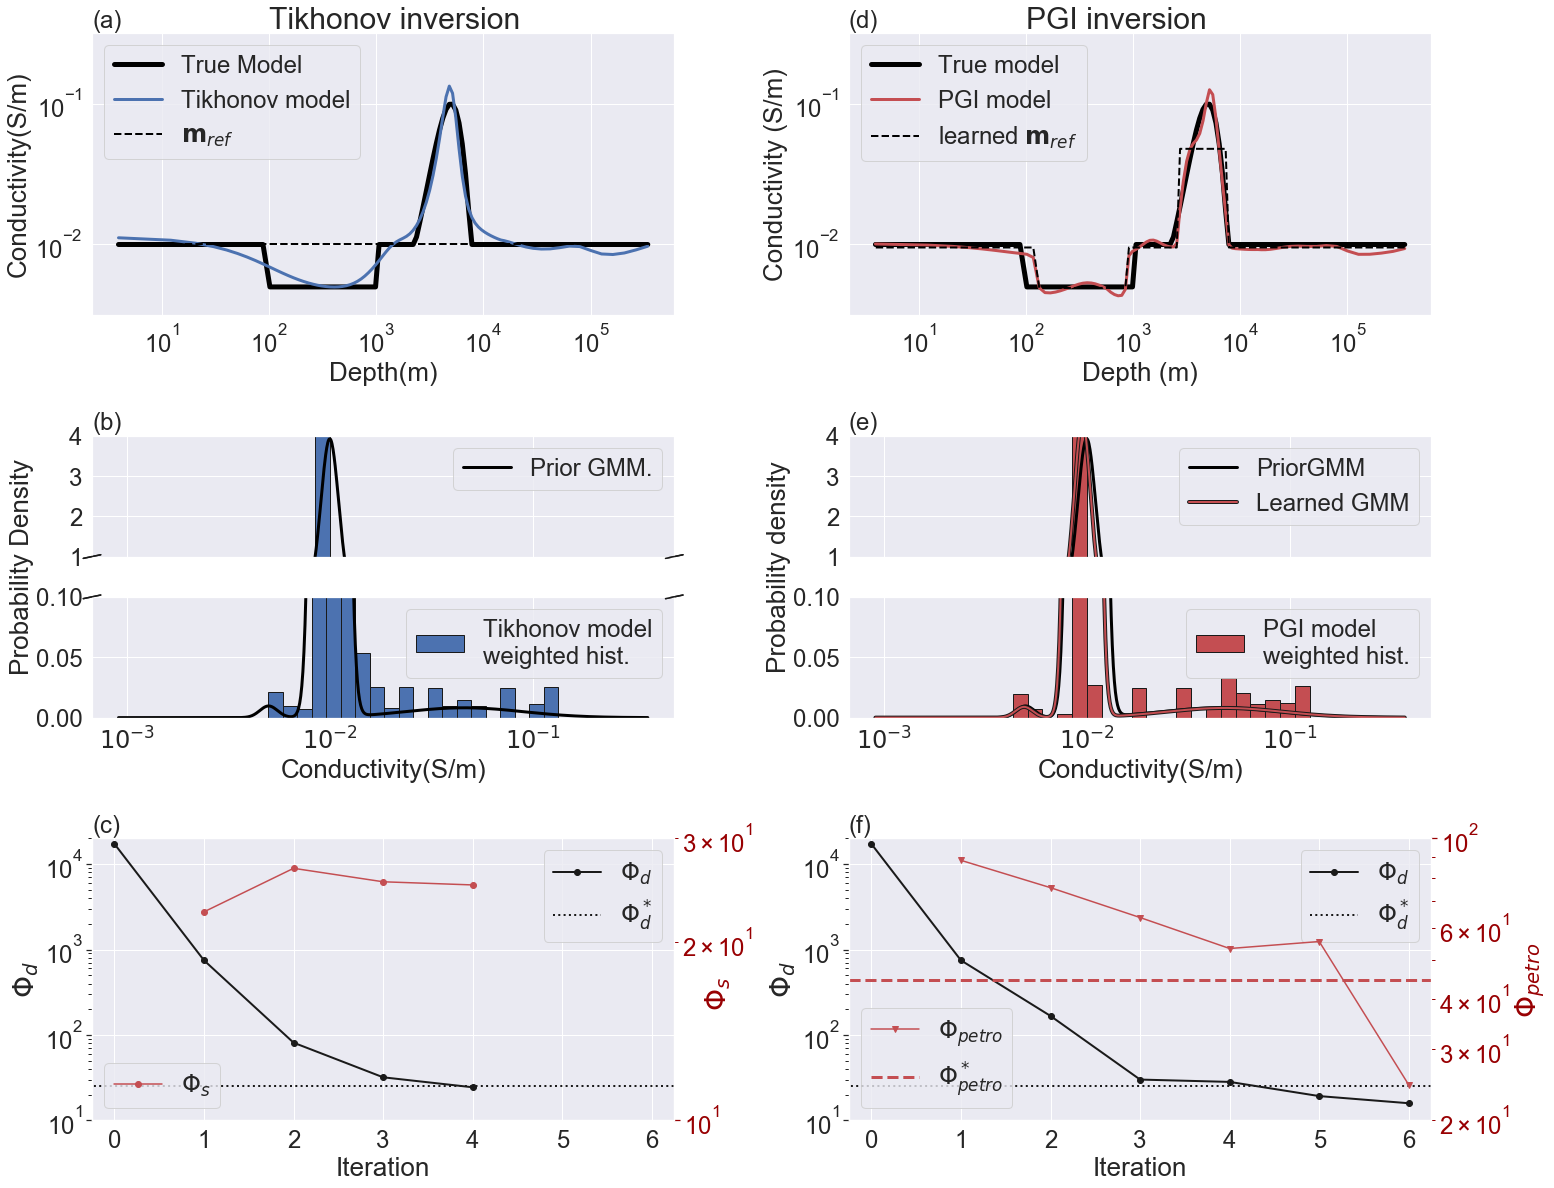
\includegraphics[width=\textwidth]{Fig/LowRes/MT1D_Results.png}
    \caption[]{MT1D example results and comparison: Figs (a), (b) and (c) show the recovered geophysical model, its histogram and the convergence curves respectively for the Tikhonov approach. Figs (d), (e) (f) shows the same plots for the PGI approach.}
 \label{fig:MT1D_smooth}
\end{figure*}

The results of the Tikhonov and PGI algorithms are shown in Fig. \ref{fig:MT1D_smooth}. The Tikhonov model is presented in Fig. \ref{fig:MT1D_smooth}(a) and the PGI model is shown in Fig. \ref{fig:MT1D_smooth}(d). The Tikhonov inversion is smooth everywhere, but character of  units blockiness or smoothness are much better recovered in the PGI model. Note that both algorithms started from the same reference model. This reference model is kept constant in the Tikhonov approach whereas the PGI algorithm updates it, along with the smallness weights, at each iteration.

The PGI recovered petrophysical distribution (Fig. \ref{fig:MT1D_smooth}e) is also much closer to the prior and true distributions, compared to the Tikhonov result (Fig. \ref{fig:MT1D_smooth}b). The means, variances and proportions of each unit are well recovered. Despite the fact that we used only confidences of unity in the prior GMM parameters, we were able to recover a learned petrophysical distribution that was close to the true distribution. The recovered variance of the background is ($7.2 \cdot 10^{-3}~[\ln(\text{S/m})]^2$). This is less than our prior value of $0.01[~\ln(\text{S/m})^2]$. This means that we recovered a background conductivity with a smaller variance than the one prescribed by the prior.

In addition to being closer to the ground truth, our inversion procedure converges in a similar manner as the Tikhonov approach (Figs \ref{fig:MT1D_smooth}c and f). The PGI method took only two additional iterations, compared to the Tikhonov approach, to reach the geophysical and petrophysical target misfits (shown respectively in black and red in Fig. \ref{fig:MT1D_smooth}f). They are reached respectively at the fifth and sixth iterations. Those two Figs \ref{fig:MT1D_smooth}(c) and (f) also highlight that the smallness is now a term to be minimized in the PGI. In Tikhonov we are unconcerned about the value of $\Phi_s$ and it usually increases when $\beta$ decreases. In PGI, $\Phi_s$ measures how well the petrophysical and geological information are recovered.

\subsubsection{Step-by-step of the PGI iterations}

\begin{figure*}
\centering
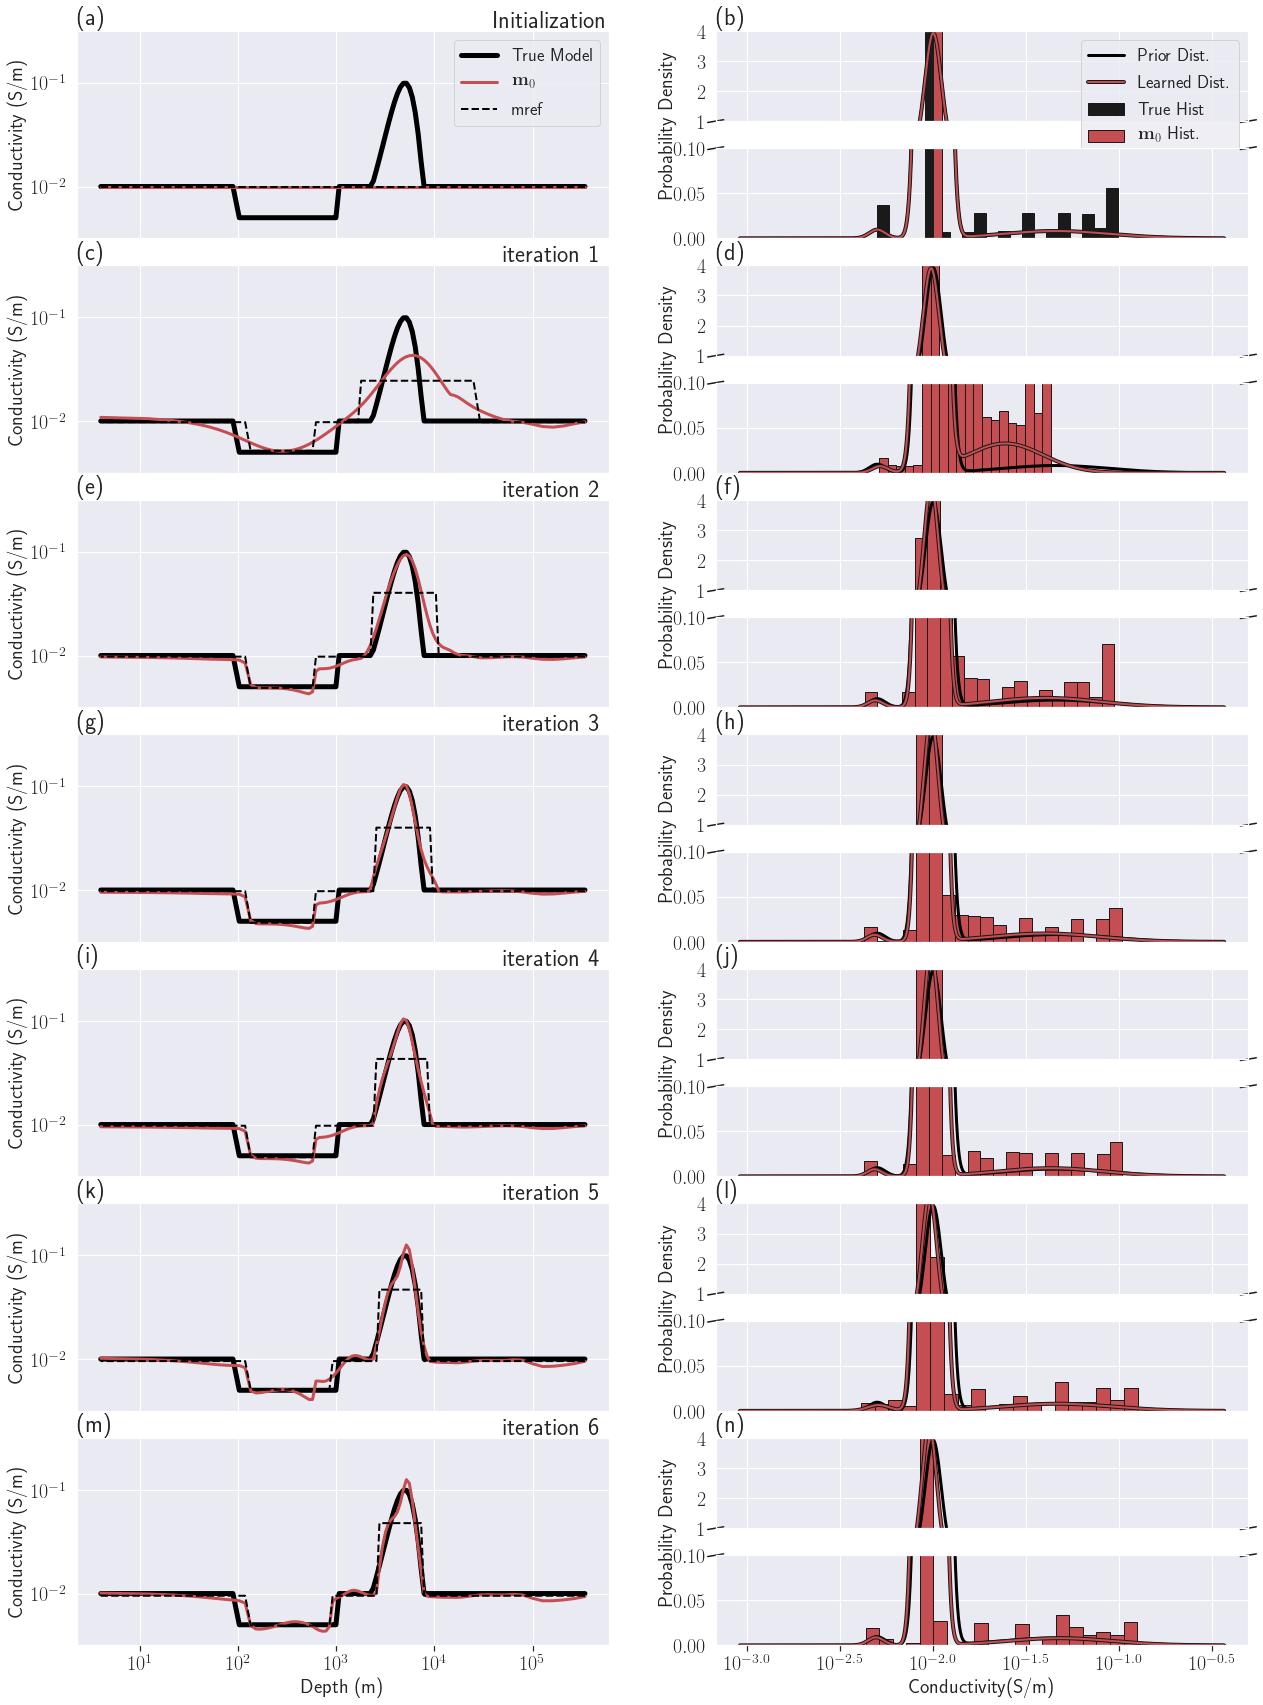
\includegraphics[width=0.95\textwidth]{Fig/LowRes/MT1D_Iterations.png}
\caption[]{Iterations of the PGI MT1D example}
\label{fig:MT1D_Iterations}
\end{figure*}

The iterations of the PGI are shown in Fig. \ref{fig:MT1D_Iterations}. Figs \ref{fig:MT1D_Iterations}(a) and (b) show our initialization. The initial and reference model is a half-space with a conductivity equal to the background conductivity. The prior and initial petrophysical distribution $\Theta_{\text{prior}}$ was described in the initialization section for this example. The first iteration (Figs \ref{fig:MT1D_Iterations}c and d) is the same as the first Tikhonov iteration and the current recovered geophysical model is fairly smooth. In the Tikhonov inversion, the reference model remains the same throughout the inversion but in the PGI, the reference model and smallness weights are updated at the end of each iteration. The updated reference model is determined from the learned petrophysical distribution applied to the current geophysical model, as described in equations \ref{membership} to \ref{Ws_update}. The recovered petrophysical distribution at this first iteration already distinguishes three units but displays higher variances than the prior. The conductivity contrasts are underestimated but the overall geological classification is correct. The recovered geophysical model after the second step (Figs \ref{fig:MT1D_Iterations}e and f), with the updated reference model and smallness weights from the previous step, starts to display the desired features both spatially and in its physical property distribution; we see a sharper resistive unit and smoother conductive unit. The geophysical target misfit is reached at iteration 5 (Fig. \ref{fig:MT1D_Iterations}k and l) and the parameter $\alpha_s$ is increased. In one further step (Figs \ref{fig:MT1D_Iterations}m and n) both the geophysical and petrophysical target misfits are reached. The last iteration successfully clustered the model values while conserving $\Phi_d\leq\Phi_d^*$. The sharp contrast of the resistive unit is well recovered as well as the smoothness of the conductive unit. The learned petrophysical distribution is very close to the prior distribution. It also has a lower variance for the background unit compared to its prior value, and thus is closer to the truth.


\subsection{DC2D, buried cylinders: Working with missing petrophysical information and adding geological information} \label{DCexample}

In this example we illustrate the performance of our framework when no physical property mean values are available, and compare it to the result when full petrophysical information is available. We then show how geological information, such as depth and thickness, can be incorporated.

\begin{figure*}
\centering
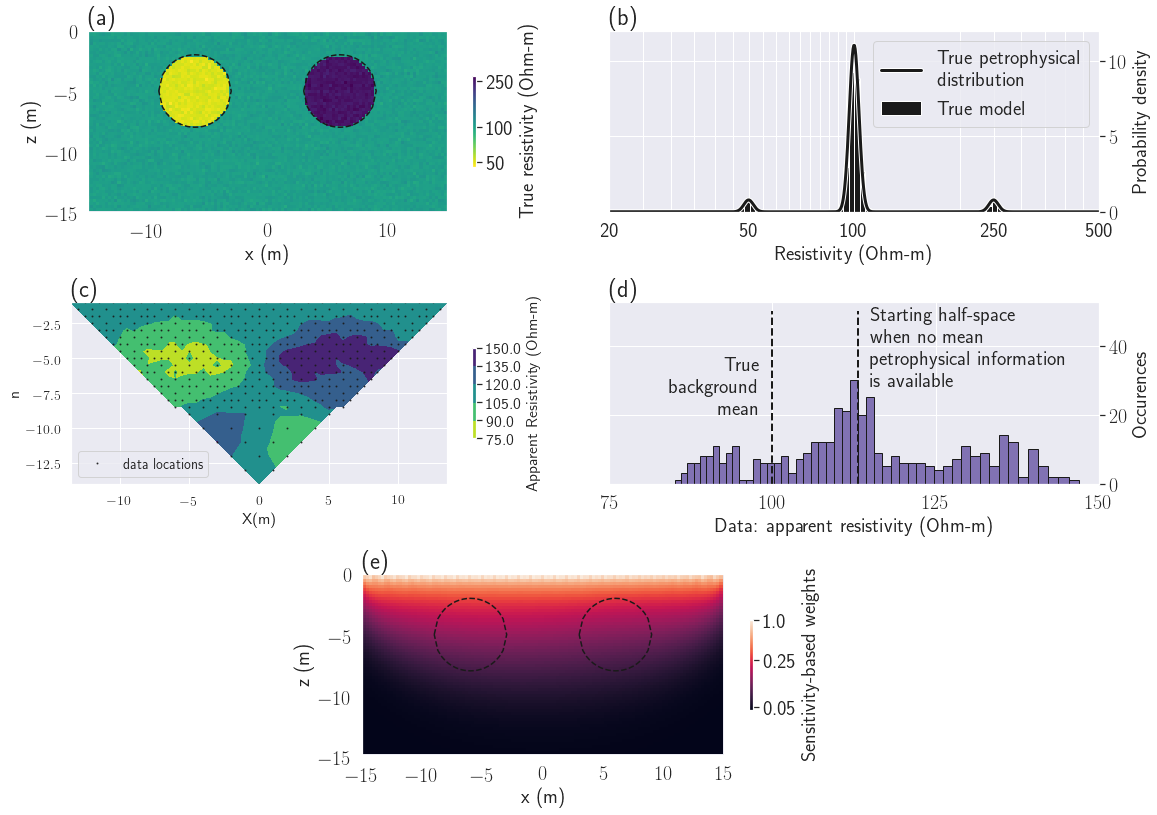
\includegraphics[width=\textwidth]{Fig/LowRes/DC2p5D_Setup.png}
\caption[]{Setup of the DC resistivity example. (a): True conductivity. (b): True petrophysical distribution. (c): DC data to be inverted. (d): Histogram of the measured apparent resistivity. The best fitting half-space ($112~\Omega \text{m}$) is indicated by the vertical dashed line. (e): Sensitivity weights $\mathbf{w}$ used for all inversions.}
\label{fig:DC2p5D_Setup}
\end{figure*}


\subsubsection{Setup}

We apply our procedure to a 2.5D DC resistivity problem (2D geology but 3D sources) to recover two cylindrical units, one conductive (with a mean resistivity of $50~\Omega \text{m}$), one resistive (with a mean resistivity of $250~\Omega \text{m}$) embedded in a background unit with a mean resistivity of $100~\Omega \text{m}$ (see Fig. \ref{fig:DC2p5D_Setup}a). To make the model slightly more geologically realistic, we added Gaussian noise to the log-conductivity model. The noise had zero mean and a variance of $1\cdot10^{-3}~[\ln(\text{S/m})]^2$ (see Fig. \ref{fig:DC2p5D_Setup}b).

Our survey is a dipole-dipole with electrode separation of $1~\text{m}$ and $2~\text{m}$ (Fig. \ref{fig:DC2p5D_Setup}c). The maximum dipole separation is set to $n=16$. We simulate a total of $419$ resistance measurements. Unbiased Gaussian noise, with a standard-deviation of $2\%$ of the original value, is added to the forwarded geophysical data. A histogram of the apparent resistivity data is shown in Fig. \ref{fig:DC2p5D_Setup}(d).

For the inversion we limit our active cells to the region covered by the survey data as shown in Fig. \ref{fig:DC2p5D_Setup}(a). The active mesh is composed of $7021$ cells. For the geophysical data misfit uncertainties, we used a floor value of $10^{-4}~V/I$ in addition to the $2\%$ noise standard-deviation.

For all of the inversions we used a sensitivity weighting that is similar to that developed in \cite{doi:10.1190/1.1820468}. This is used in place of the usual smoothing weights at the surface to compensate for the high sensitivities near electrodes. Those weights are shown in Fig. \ref{fig:DC2p5D_Setup}(e). We use $\Phi_d$ and $\Phi_{petro}$ as stopping criteria. To illustrate functionality, we also incorporated the learned reference model in the smoothness term of the geophysical objective function. This was done towards the end of the inversion, after the reference model was stabilized and $\Phi_d^*$ was reached (see algorithm \ref{algo:algorithm}, step 6).

To set benchmarks for the inversion results, we first carry out a Tikhonov inversion and a PGI with full petrophysical information. We then run a PGI without providing any information about the physical property mean values or the proportions. We finally run another PGI, still without means information, but with added geological information included through the use of local proportion weights in the GMM. All inversions start with the same geophysical objective function.

\begin{figure*}
\centering
\includegraphics[width=\textwidth]{Fig/LowRes/DC2p5D_Result.png}
\caption{DC inversion results. The color scale is the same as for the true model in Fig. \ref{fig:DC2p5D_Setup}(a). Figs (a), (b) and (c) present the recovered model, histogram and convergence curves respectively for the Tikhonov approach. Figs (d), (e) and (f) show the same plots for PGI, when the true petrophysical distribution was provided. Figs (g), (h) and (i) show the results for PGI, when no information on the proportions or the physical property means of the units were provided. Figs (j), (k) and (l) show how PGI, with no mean information, can be improved by adding information about the  depth and thickness of the cylinders.}
\label{fig:DC2p5D_Result}
\end{figure*}

\subsubsection{Tikhonov inversion}

The Tikhonov inversion starts from the best fitting half-space of $112~\Omega \text{m}$, instead of the true background value of $100~\Omega \text{m}$ (see Fig. \ref{fig:DC2p5D_Setup}d). The inversion produces the result presented in Fig. \ref{fig:DC2p5D_Result}(a). The two bodies are detected but their edges are smoothed. This smoothness is also visible in the histogram of the model that is characterized by continuous values centered on the starting half-space value (Fig. \ref{fig:DC2p5D_Result}b). The conductivity values do not attain the true electrical conductivity of the anomalies. The geophysical target misfit is reached in six iterations (Fig. \ref{fig:DC2p5D_Result}c). The parameter $\beta$ was cooled at each iteration and the smallness term kept increasing; this is expected in the Tikhonov approach.


\subsubsection{PGI with full petrophysical information}

In this example we first want to establish a benchmark result by using the true petrophysical distribution with global proportions. We fix the petrophysical distribution at the true one (Fig. \ref{fig:DC2p5D_Setup}b) by setting all our confidences in the petrophysical prior to infinity. Thus $\Theta=\Theta_{\text{prior}}=\Theta_{\text{true}}$ is fixed for all iterations. We start from a half-space with the true mean background value.

This benchmark inversion recovers the two cylinders (Fig. \ref{fig:DC2p5D_Result}d) quite well. The locations of the cylinders, their outer boundaries and their conductivities are in reasonable agreement with the true model. The geophysical model also satisfactorily fits the true petrophysical distribution being imposed (Fig. \ref{fig:DC2p5D_Result}e). The geophysical target misfit is reached after seven iterations (Fig. \ref{fig:DC2p5D_Result}f). An additional seven iterations is needed to reach the petrophysical target misfit, while keeping $\Phi_d\leq\Phi_d^*$. The two increases of $\Phi_{petro}$ seen at iteration $3$ and $7$ correspond to $\beta$-cooling.  This was necessary since the geophysical misfit was not decreasing enough (see algorithm \ref{algo:algorithm}, step 6). The important decrease seen at iteration $11$ corresponds to the inclusion of the learned reference model in the smoothness. This helps us reach the petrophysical target misfit. This highlights the importance of incorporating a discontinuous reference model into the smoothness terms so that large gradients in the model are not penalized. This allowed for the final model to have sharp boundaries which is consistent with the true model.

\subsubsection{PGI with no physical property means information}

We now consider the situation where no prior information is known, except the expected number of units (three in this example). We can still use our framework but we turn off the prior on the means and proportions. The confidences $\{\mathbf{\zeta},\mathbf{\kappa}\}$ are thus set to zero (no prior information on the means or proportions). We used the true variances with infinite confidences $\mathbf{\nu}$ in them. We thus have specified the petrophysical noise levels, which regulate how much each unit has to cluster around its unknown mean. This is analogous to choosing an appropriate geophysical data noise level. Our inversion starts from the best fitting half-space, as in the Tikhonov inversion, since the true background value is now considered to be unknown.

The recovered geophysical model still displays a clustered aspect with structures close to the ground truth (Fig. \ref{fig:DC2p5D_Result}g). The volumes of the two cylindrical units are overestimated. The histogram and model show three distinct units. Without the true means information, the recovered means of the cylinders are slightly shifted towards the background value (Fig. \ref{fig:DC2p5D_Result}h). Interestingly the recovered mean of the background is closer to the true mean than the initial half-space model. The number of iterations to reach both target misfits is comparable to the PGI example that used full petrophysical information.


\subsubsection{PGI with geological information}

Our next goal in this example is to illustrate how geological information might be included. It is motivated by the fact that, in the two previous PGI results (using full and no petrophysical information), the cylindrical units display various size anomalies compared to the ground-truth and extend to different depths. Suppose information about the anomalous zone's depth and thickness are provided. This additional information can be added to the inversion through local proportion parameters $\mathcal{P}(\mathbf{z})$, by making them vary with depth. At depths where the anomalous bodies are expected, we set equal prior expectation of encountering any of the three units (so here $\pi=1/3$ for all three units for locations at depth between $2~\text{m}$ and $8~\text{m}$). At depths where only the background is expected, we set $\$\mathcal{P}(\mathbf{z}=\text{background})=1$ and $\mathcal{P}(\mathbf{z}=\text{cylinders})=0$. Those proportions are summarized in table \ref{proportions_depth}. We used this prior information in a new PGI, using the petrophysical distribution recovered from the PGI with no mean information as $\Theta_{\text{prior}}$.

\begin{table}
 \caption{Proportions of the GMM $\mathcal{P}(\mathbf{z})$ as a function of depth to include geological information. Legend: Bckgrd: background; cond.: conductive unit; res.: resistive unit.}
 \label{proportions_depth}
 \begin{tabular}{@{}lcccccc}
\hline
  Depth range (m) & $\mathcal{P}(\mathbf{z}=\text{bckgrd})$ & $\mathcal{P}(\mathbf{z}=\text{cond.})$ & $\mathcal{P}(\mathbf{z}=\text{res.})$ \\
\hline
  $\leq 2$ & $1$ & $0$ & $0$ \\
  $2-8$ & $1/3$ & $1/3$ & $1/3$ \\
  $\geq 8$ & $1$ & $0$ & $0$\\
\hline
 \end{tabular}
\end{table}

The recovered model (Fig. \ref{fig:DC2p5D_Result}j) is similar to the PGI with no petrophysical information except the anomalies are now restricted to the right depths. Comparing the two learned distributions, with and without depth information, we notice that the recovered conductivity values from the PGI model with geological information are closer to the ground-truth than the conductivities recovered from the PGI with no petrophysical or geological information (Fig. \ref{fig:DC2p5D_Result}k). The convergence of the algorithm is similar to the previous PGIs (Fig. \ref{fig:DC2p5D_Result}l).


%%%%%%%%%%%%%%%%%%%%%%%%%%%%%%%%%%%%%%%%%%%%%%%%%%%%%%%%%%%%%%%%%%%%%%%%%%%%%%%
\subsection{Using PGI to reduce ambiguity: a field example} \label{section:field_data}

In any inversion the final result is affected by many terms and parameters in the objective function, but of particular interest here is the choice of reference model. In a Tikhonov inversion starting from different half-space reference models can lead to different solutions, and this complicates the interpretation. Some of the ambiguity might be reduced if more information is incorporated. The PGI approach allows us to add information, such as a desired number of geological units, that are otherwise difficult to use in a Tikhonov setting. Adding a constraint on the number of units we wish to recover, without incorporating other extensive geological or petrophysical information, can be enough to reduce the realm of possible models.

We illustrate this on a field frequency-domain EM dataset \citep{WardandHohmann} for saline water delineation. We begin by emphasizing the discrepancies seen in Tikhonov models using different half-space reference models. We then show that by using PGI and assuming an expected number of distinct units, that starting from different reference models leads to similar inversion results that have consistent petrophysical distributions and simplified structures. The lack of dependence upon the initial and initial reference models helps to build confidence in the final images.

\subsubsection{Setup}

\begin{figure*}
    \centering
    \includegraphics[width=\textwidth]{Fig/LowRes/Booky_setup.png}
    \caption[]{Bookpurnong survey area. The elevation of the survey area is represented as an overlaid colormap. The white arrows represent the water flow, both of the river and from the irrigation zone. Geographic system: WGS 84 / UTM 54S. Aerial images from Google Earth, \textcopyright2019 DigitalGlobe.}
    \label{fig:Book_Setup}
\end{figure*}

The Bookpurnong irrigation District is part of the Riverland region of South Australia along the Murray river. The irrigation on the highland river bank has lead to the salinization of the floodplain soil and threatens to make the area inhospitable for vegetation (Fig. \ref{fig:Book_Setup}). The key issue is to determine if (and where) the fresh water river is charging the aquifer (called "losing stream", this is the healthy scenario), or if the saline aquifer is charging the river, and thus contaminating the floodplain soil ("gaining stream" scenario). To help the work of hydrogeologists, various frequency and time-domain electromagnetics surveys have been conducted to characterize saline zones which are diagnosed by an increase in electrical conductivity. High conductivities close to the surface will indicate a "gaining stream" scenario while low conductivities will be a sign of a "losing stream".

The Bookpurnong case study has been studied in previous publications \citep{Bookpurnong,viezzoli2010,Yang2017}. Here we focus on the RESOLVE frequency domain dataset, flown in 2008, which covers an area of approximately $6,650~\text{m}$ by $2,400~\text{m}$.

At each sounding, the RESOLVE system measures the real and imaginary parts of the induced magnetic field for $5$ frequencies ranging from $382~\text{Hz}$ to $130.1~\text{kHz}$. The survey consists of 1022 soundings, resulting in a total number of data of $10,220$. For the geophysical noise levels, we use a standard-deviation of $10\%$ of the absolute value of the datum and add a $20~\text{ppm}$ floor value; this is consistent with previous studies.

\subsubsection{Inversion setup}

To invert the RESOLVE dataset, we choose a laterally-constrained 1D approach similar to \cite{Viezzoli2008} using the EM1D module of the SimPEG package \citep{heagy2017framework,SimPEGEM1DPoster}. Each sounding is inverted in 1D using a mesh with 19 layers that extends to a depth of $187~\text{m}$. The cells increase in size from $2.5~\text{m}$ at the surface to $25~\text{m}$ for the last layer. We use the thickness of the layers as weights in the regularization, which relates to an integral formulation of the regularizer \citep{doi:10.1190/1.9781560801719.ch5}.

For each Tikhonov and PGI approach, we run two separate inversions using $0.01~\text{S/m}$ ($100~\Omega \text{m}$) and $1~\text{S/m}$ ($1~\Omega \text{m}$) models respectively as reference models (thus four inversions are carried out). The reference models are also used as initial models $\mathbf{m}_0$. The reference model stays the same throughout the Tikhonov inversions while the PGI algorithm updates it.

\subsubsection{Tikhonov inversions}

\begin{figure*}
\centering
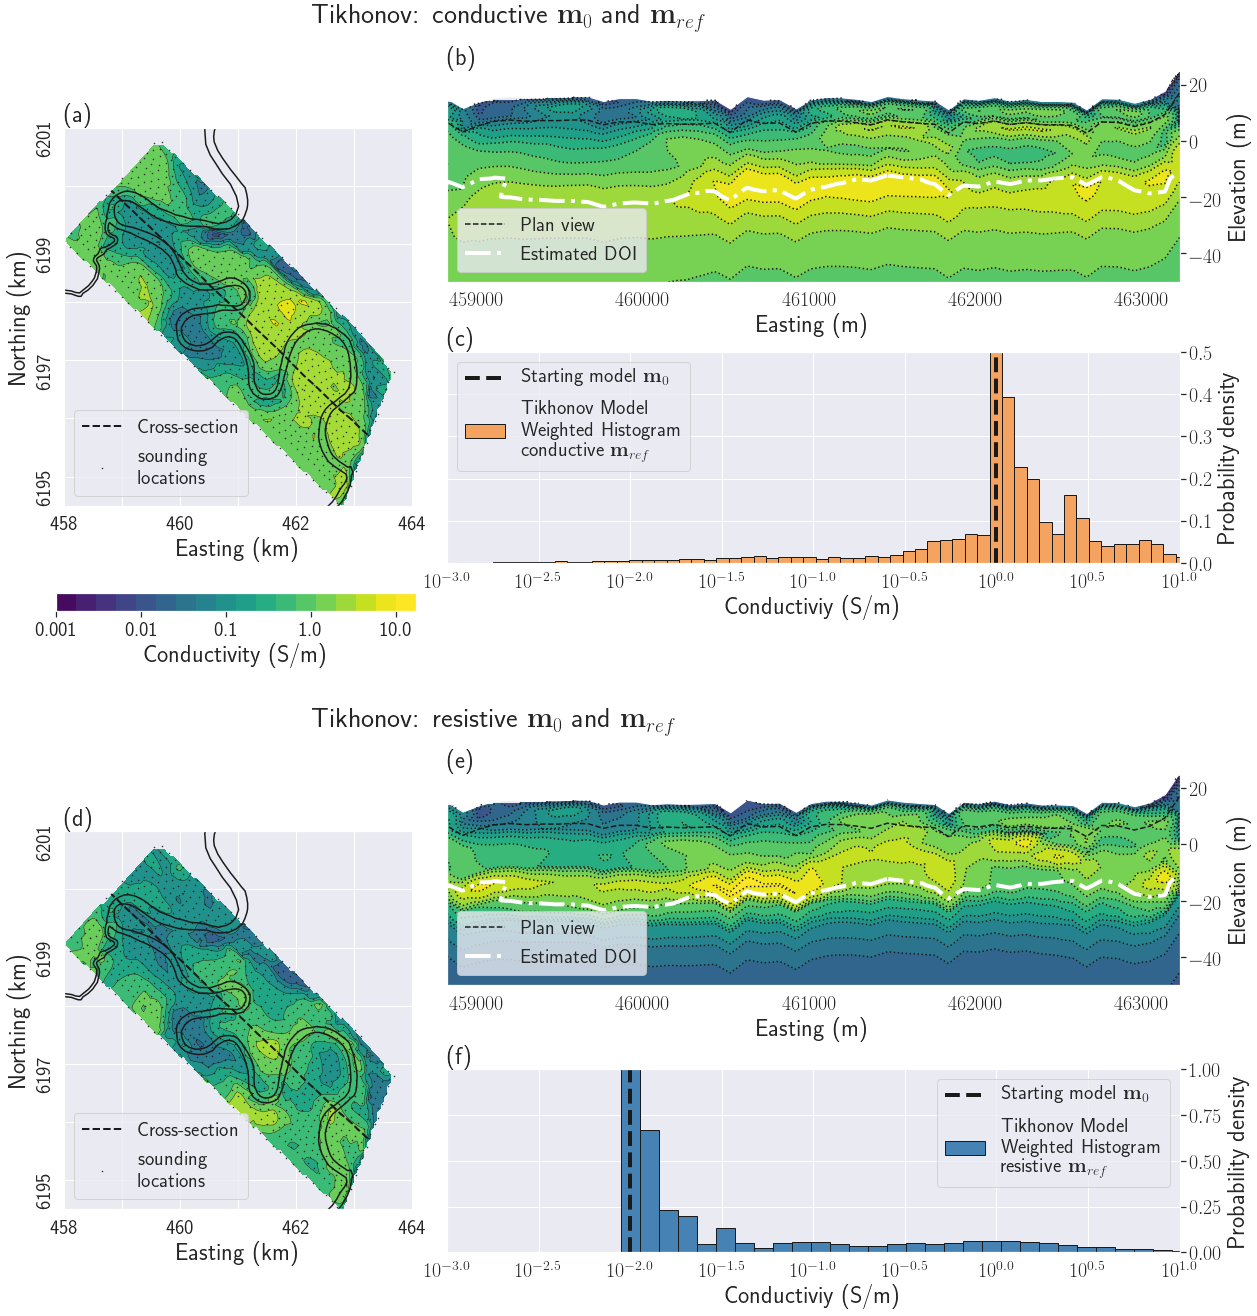
\includegraphics[width=\textwidth]{Fig/LowRes/Booky_L2_Results.png}
\caption{Tikhonov results with two different reference models. All figures share the same color scale for conductivity. Figs (a), (b) and (c) show the results starting from a conductive half-space. Figs (d), (e) and (f) show the result starting from a resistive half-space. Figs (a) and (d) display the recovered geophysical models on a plan view at a depth of $8.5$ m. Figs (b) and (e) display a cross-section of the recovered geophysical models. Depth of investigation (DOI) evaluated using the method presented in \cite{DOI}. Figs (c) and (f) display the histogram of the recovered model for each inversion.}
\label{fig:Book_L2_Results}
\end{figure*}

The results of the Tikhonov inversions using two different reference models are summarized in Fig. \ref{fig:Book_L2_Results}. Both Tikhonov models (Figs \ref{fig:Book_L2_Results}a and d) detect the river at the surface as a resistive feature; it is also visible where the cross-section crosses the river near $459~$,$459.8~$, $460.5$, $461$, $461.8$ and $462.5$ km on Figs\ref{fig:Book_L2_Results}(b) and (e). Both models also pick up highly conductive features at depth and the laterally-constrained regularization helps ensure horizontal continuity. The ranges of conductivity are similar to those observed in boreholes \citep{BookyExperiment}.

In the north-west part of the area, the recovered conductivity models are consistent and transition smoothly from resistive at the surface to conductive at depth. In the south-east part of the area, more discrepancies in the two models are visible (see section \ref{pgitikcomparison} for a quantification of the discrepancies). On the plan views (Figs \ref{fig:Book_L2_Results}a and d), the overall recovered conductivities in the biggest bend in the river are an order of magnitude different between the two inversions. Inconsistent pocket-like structures are seen in both inversions in the cross-sections (Figs\ref{fig:Book_L2_Results}b and e). Both cross-sections however show that the conductive layer is closer to the surface in the South-East than in the North-West.

\subsubsection{PGI}

We now apply the PGI approach without providing specific petrophysical information; only the number of units is specified. We show that similar geophysical models and petrophysical distributions are obtained even though the inversions are carried out with different initial reference models.

As we did for the Tikhonov inversions, we now run two inversions starting from uniform $0.01~\text{S/m}$ ($100~\Omega \text{m}$) and $1~\text{S/m}$ ($1~\Omega \text{m}$) models respectively, used as initial and initial reference models. For the conductive and resistive reference model cases respectively, both the Tikhonov and PGI approaches start with the same objective function; the models after the first iteration are thus identical.

For the prior petrophysical distribution, we do not specify any prior value for the mean conductivity values nor the proportions; their respective confidence parameters are thus set to zero. We choose variances of $0.1 [\ln(\text{S/m})]^2$. We set the confidences in the prior covariances to unity. Our goal with this choice is to recover a model with distinct units but still reasonably smooth. %to recover a model with distinct units but still with reasonably smooth contrast.

A critical point here is to choose the number of distinct units we want to recover. We assume that there are three units, as this matches our interpretation goal of distinguishing freshwater from salinized water, with an additional transition zone. This adds an additional constraint on the models we want to recover.

\begin{figure*}
\centering
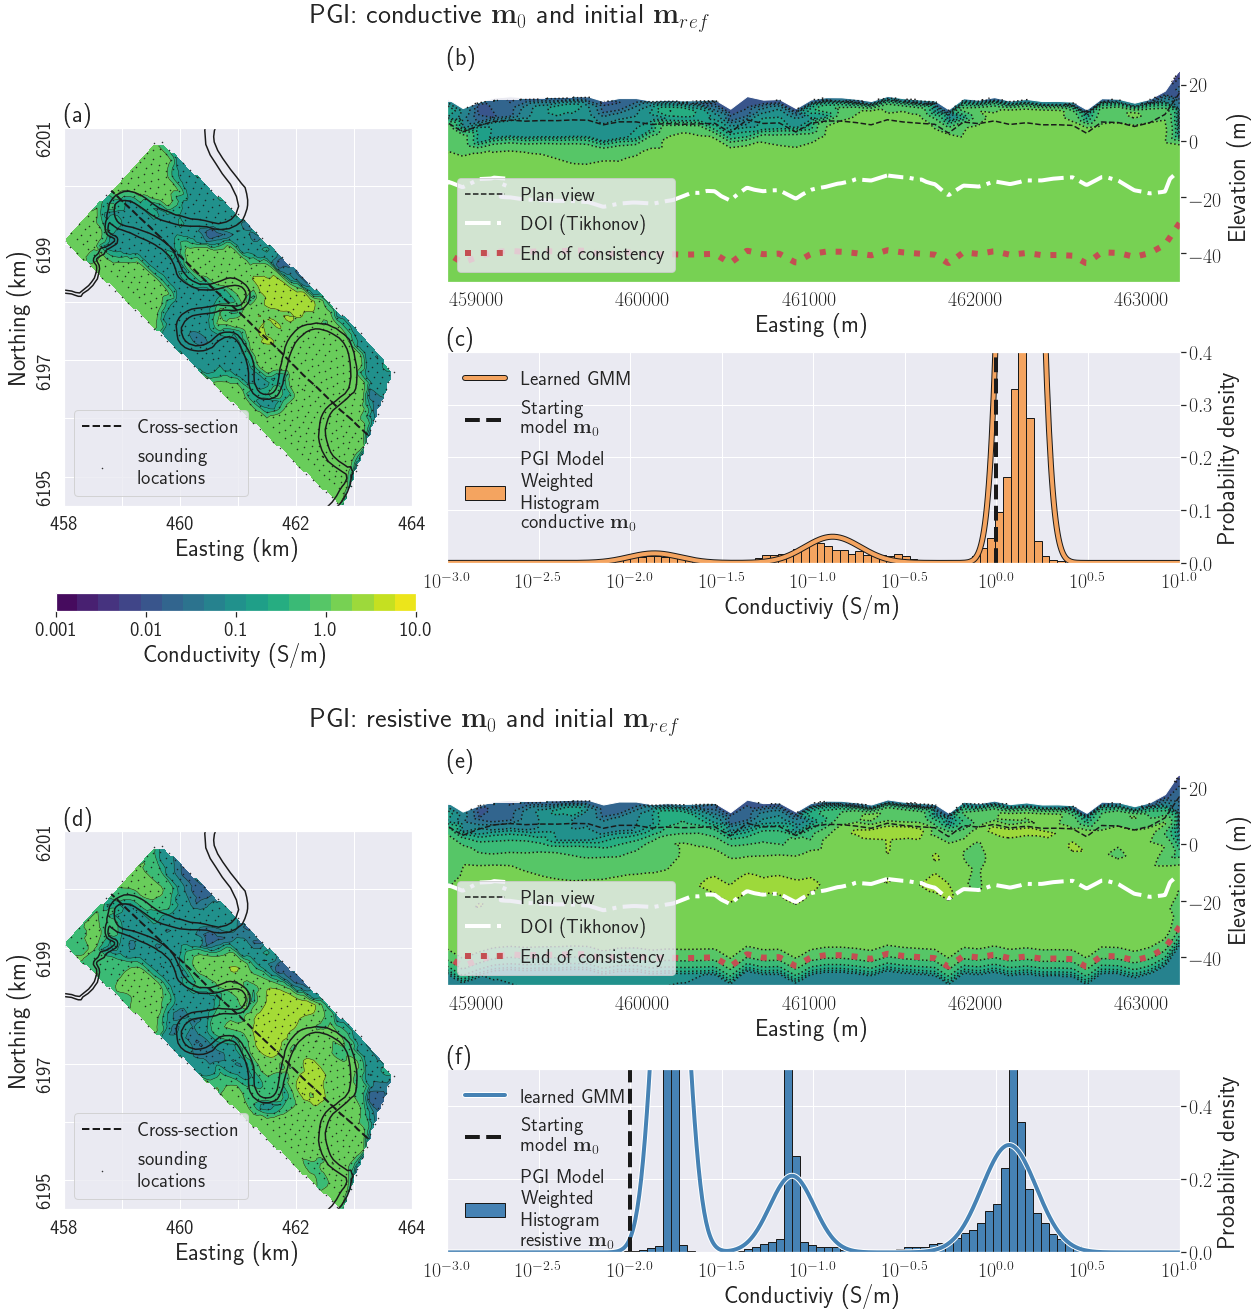
\includegraphics[width=\textwidth]{./Fig/LowRes/Booky_pgi_result.png}
\caption{PGI results with two different initial and initial reference models. All figures share the same color scale for conductivity. Figs (a), (b) and (c) show the results starting from a conductive half-space. Figs (d), (e) and (f) show the results starting from a resistive half-space. Figs (a) and (d) display the recovered geophysical models on a plan view at a depth of $8.5$ m. Figs (b) and (e) display a cross-section of the recovered geophysical models. Figs (c) and (f) display the histogram of the recovered model and the learned petrophysical distribution for each inversion.}
\label{fig:Book_PGI_Results}
\end{figure*}

The PGI results are compiled in Fig. \ref{fig:Book_PGI_Results}. All PGI have reached their geophysical and petrophysical misfits. The recovered models (Figs \ref{fig:Book_PGI_Results}a and \ref{fig:Book_PGI_Results}d) are more consistent with each other than those in the Tikhonov case; we will discuss this later in section \ref{pgitikcomparison}.

Counterintuitively, by clustering the histograms we actually smoothed the resulting model by forcing more homogeneity inside each distinct unit. Neither cross-section (Figs \ref{fig:Book_PGI_Results}b and e) shows the pocket-like structure in the south-east end of the profile that were observed in the Tikhonov inversions; it indicates that those features were not robust. The high conductivity layer is closer to the surface in the South-East than in the North-West in both models.

The histograms and recovered petrophysical distributions (Figs \ref{fig:Book_PGI_Results}c and f) display several interesting characteristics. First we recover three distinct units that can be interpreted as fresh, transition and saline zones. The learned means of the clusters are very similar between the two inversions. We notice that in the case of the resistive initial models, the resistive unit conductivity has been corrected to about $0.017~\text{S/m}$ ($60~\Omega \text{m}$). The same phenomenon happens for the conductive initial models case, with a corrected conductive unit conductivity value of $1.35~\text{S/m}$ ($0.74~\Omega \text{m}$). This behavior was noticed in the DC example (section \ref{DCexample}) when starting from a biased background value. The major difference between the GMM for the two models is the variance and proportion of the most resistive and most conductive units. This is due to the volume of the region in the padding zones that are outside the region of influence of the data. The values of conductivity in those regions stays close the cluster mean which is closest to the conductivity of the initial reference model.

\subsubsection{PGI - Tikhonov comparison} \label{pgitikcomparison}

In addition to the removal of unnecessary structure mentioned earlier, the models recovered with the PGI approach display more consistent subsurfaces features than do the Tikhonov models. To quantify the similarities between models within the same methodology but with different initial and reference models, we adopt an approach analogous to the depth of investigation (DOI) estimation presented in \cite{DOI}. For the two Tikhonov and the two PGI conductivity models respectively, which for clarity in the notation are referred to in the following equation as electrical resistivity $\mathbf{\rho}_1$ and $\mathbf{\rho}_2$, we computed their maximum ratio $\mathbf{r}$ everywhere:

\begin{align}
\mathbf{r} = \mathop{\hbox{max}}(\frac{\mathbf{\rho}_1}{\mathbf{\rho}_2},\frac{\mathbf{\rho}_2}{\mathbf{\rho}_1})~(1\leq r \leq \infty)
\end{align}

A ratio $r$ of unity indicates similar values of conductivity. The higher the value of $r$, the more the two models differs. Fig. \ref{Booky_compare} shows the result of this two-by-two comparison. The two PGI models are quite consistent, with ratio $r$ values close to unity almost everywhere, except in a small area in the North-West. On the contrary the Tikhonov inversions show significant discrepancies, even in the near-surface, with $r$ values greater than $2$ in most of the survey area. This is especially visible near the important bend in the river in the South-East where discrepancies of more than an order of magnitude ($r\geq10$) are observed (dark areas in Fig. \ref{Booky_compare}). Fig \ref{Booky_compare}(j) highlights when the Tikhonov inversions reached their DOI and where the final model is controlled mostly by the regularization. It is worth noticing that the PGI models are still consistent past the DOI estimated from the Tikhonov inversions (Figs \ref{fig:Book_PGI_Results}b and e).

\begin{figure*}
\centering
\includegraphics[width=\textwidth]{./Fig/LowRes/Booky_ratio_compare.png}
\caption[]{Consistency comparison between the two Tikhonov and the two PGI models, starting with conductive and resistive initial and reference models. The first row displays the ratio $r$ of the two PGI conductivity models at different depths. The bottom displays the same ratio for the two Tikhonov conductivity models. Depths of the plan views increase from left to right. Pale yellow means the two conductivity models differ by less than a factor 2. Orange highlights areas where the recovered conductivities differ by more than a factor 2. Dark purple emphasizes area where the two  recovered conductivity models differ by more than a factor 10.}
\label{Booky_compare}
\end{figure*}

\subsubsection{Field example summary}

We demonstrated that even in the near-surface above the depth of investigation the Tikhonov inversions had different structures when different initial and reference models were used. With the PGI approach, the two inversion lead to similar near-surface models that have consistent petrophysical distributions. The removal of structures, evidently not required by the data, and the simplification of the geology, provides a result that is more appealing to interpret geologically. Making a reasonable guess about the variances and the number of units were the crucial additional information required to achieve this. All four models point to a "losing stream" scenario in the North-West while three (both PGI models and the Tikhonov inversion with a conductive reference model) indicate a "gaining stream" in the South-East. This is coherent with the conclusions given in \cite{Bookpurnong,viezzoli2010} and \cite{Yang2017}. To further extend our analysis, ground-truthing the depth of the saturation salinization zone and adding it into the PGI as geological information, or adding petrophysical measurements, would be required.

%%%%%%%%%%%%%%%%%%%%%%%%%%%%%%%%%%%%%%%%%%%%%%%%%%%%%%%%%%%%%%%%%%%%%%%%%%%%%%%
\section{Discussion}

We have presented a framework for carrying out a petrophysically and geologically guided inversion which allows the user to recover a quasi-geological rock model \citep{QuasiGeologicalModel} and a petrophysical distribution in addition to the geophysical model. The framework has three main modules, each of which is formulated as a MAP estimate. The framework is flexible and goals, achieved by others and using different approaches, can be incorporated while the reverse is not true.

Carrying out an inversion that includes three separate sub-problems that communicate with each other, and for which two target misfits are to be achieved, is challenging. To address this we have provided a pseudocode as well as a flowchart in appendix \ref{section:pseudocode}. The important part of the procedure is the initialization step where the user must specify what is known, how to incorporate it, and what they want as an end product. The examples explore those various aspects as well as the convergence of the PGI approach.

The crucial component of our framework is to provide a different role for the smallness component of the regularization term in the geophysical objective function. An evolving reference model, tied to different units in a GMM, ultimately allows this term to be viewed as a quantitative metric for determining how well the petrophysical and geological data are fit. This has many advantages. The inverse problem is now solved by finding a model $\mathbf{m}$ and a reference model $\mathbf{m}_{\text{ref}}$, along with the smallness weights, such that the geophysical, petrophysical and geological data are fit. This complicates the inversion but the procedure is greatly simplified compared to adding additional terms, along with their adjustable hyperparameters, in the regularization. This also allows this research to be incorporated with other developments done using the Tikhonov approach. For example when sharp contrasts are expected, such as in the DC example developed in section \ref{DCexample}, the effects of using sparse norms for the model gradients in the smoothness term \citep{SparseNorms2} are worth exploring. This would allow the combined use of petrophysical and structural data to guide the inversion.

Our solution is achieved by first focusing on the geophysical data misfit and solving the optimization problem at successively smaller values of the global trade-off parameter $\beta$. In some cases, finding an acceptable model to the geophysical data also makes the petrophysical misfit sufficiently small. If it doesn't, then we adjust $\alpha_s$ which controls the relative weight between the smallness and the other components of the objective function. So far our heuristic approach has worked satisfactorily but searching simultaneously for optimal $\beta$ and $\alpha_s$ values such that both $\Phi_d(\mathbf{m})\simeq\Phi_d^*$ and $\Phi_{petro}(\mathbf{m})\simeq\Phi_{petro}^*$ is a more advanced optimization process and deserves further research. For example \cite{BetaAlphaEstimation} is entirely dedicated to the problem of refining the values of $\beta$ and $\alpha_s$ within the FCM-guided inversion approach \citep{Sun2015}, and only for magnetic linear problems.

Further work is also required about the best way to evaluate the petrophysical target misfit. In our framework we minimize $\Phi_s$ which is a weighted petrophysical misfit. Those weights are usually related to the physics of the survey and they are often necessary for solving inverse problems where sensitivities are greatly varying (e.g. in potential field data). Since we know the weights, we can evaluate $\text{E}\lbrack\Phi_s\rbrack$ and use that as a fitting criterion. Another option is to evaluate$\Phi_{petro}$; this amounts to evaluating $\Phi_s$ without weights. Both have worked for us, but working with $\Phi_{petro}$ has constantly produced good results and it is appealing to have a stopping criterion tied only to the petrophysical and geological characteristics of the model.

Another key component of our framework is the possibility for the algorithm to learn all the parameters of a suitable GMM distribution when little to no information is known a priori. The MAP-EM algorithm has been an essential element in achieving this goal. The minimum requirement is to provide an expected number of distinct units and a prior petrophysical noise level for each unit.

The MAP-EM algorithm with semi-conjugate priors formalizes the update of the means done in \cite{Sun2015} and generalizes it to the other GMM parameters. An important aspect of our formulation of the MAP-EM algorithm is the incorporation of the volume elements into the evaluation of the GMM parameters, rather than just working with cell-counts. Working with volumetric values ensures that our recovered GMM parameters are independent of the discretization. The estimation of the GMM parameters includes a prior weighted by our confidences in this prior, in a similar sense that we have a confidence $\beta$ in the geophysical model prior during the geophysical inversion. So far values of unity or above for the confidences in the variances have worked well whether or not we knew the true petrophysical distribution. Confidences in the means and proportions appear dependent of the quality of the prior knowledge. Effects of their values is to be further investigated, as well as if cooling or warming those parameters, similar to what is done with $\beta$, can have an impact on the recovery or convergence.

%%%%%%%%%%%%%%%%%%%%%%%%%%%%%%%%%%%%%%%%%%%%%%%%%%%%%%%%%%%%%%%%%%%%%%%%%%%%%%%
\section{Conclusions}

We have developed a framework for carrying out petrophysically and geologically guided inversions using a dynamic Gaussian mixture model prior. Importantly we achieve our goal of incorporating both geological and petrophysical information in geophysical inversions without including an additional term in the objective function. Rather, we update the reference model and the smallness weighting matrix at each iteration of the geophysical model through the optimization of posterior probability distributions. This allows our work to be compatible with previous Tikhonov approaches and readily adapted to existing inversion codes. Our flexible prior formulation allows us to refine the petrophysical model as part of the iterative process. Our inversion continues until the geophysical, geological and petrophysical data are fitted. For that purpose, we have defined a target misfit to measure how well the recovered geophysical model fits the petrophysical and geological distribution. We have presented a suite of synthetic and field examples to illustrate important aspects of our framework, especially in demonstrating how prior petrophysical and geological information is incorporated. We have also shown that detailed knowledge of the petrophysical or geological properties is not required to make significant gains in the recovered geophysical models. Our examples deal with a single physical property but our framework has been designed to carry out joint inversion of different types of geophysical data, as illustrated in \cite{Astic2018b}; this topic will be addressed in a follow-up paper.

Lastly, we comment upon how important the development of open-source software packages has been for our research. It has allowed us to benefit from the work carried out by others. The development of the MAP-EM algorithm has been facilitated by the MLE code available through the open source Scikit-Learn project, a library of tools for machine-learning \citep{scikit-learn}. The successful application of our methodology to various geophysical survey methods, such as potential fields, DC, MT or FDEM, has been made possible because of the interconnectivity of SimPEG, an open source package to carry out geophysical inversions \citep{Cockett2015,heagy2017framework,SimPEGEM1DPoster}. To ensure reproducibility of the results in this paper, and to contribute to the development of the open source community, we are making the examples presented in this paper available online \citep{PGIexamples}, through the use of Jupyter Notebooks \citep{Perez2015}. This allows researchers to readily use our framework and also to contribute to the development of inversion codes that incorporate geophysical,  geological and petrophysical data to yield meaningful solutions.


%%%%%%%%%%%%%%%%%%%%%%%%%%%%%%%%%%%%%%%%%%%%%%%%%%%%%%%%%%%%%%%%%%%%%%%%%%%%%%%
\section{Acknowledgments}

We thank Tim Munday (CSIRO) for making the Bookpurnong datasets available. We also thank all of the developers who have contributed to the SimPEG package (\url{https://simpeg.xyz}). In particular we thank Lindsey J. Heagy for her development of architectural features that allowed us to use flexible regularization functions and also to connect forward modellings that were based upon different physics, and Seogi Kang and Dominique Fournier for their implementation of the parallelized stitched EM1D code in SimPEG as well as for the many fruitful conversations. A special thanks to Rowan Cockett as a main founder of the SimPEG project, and to the entire SimPEG group for their support and for many fruitful conversations.


%%%%%%%%%%%%%%%%%%%%%%%%%%%%%%%%%%%%%%%%%%%%%%%%%%%%%%%%%%%%%%%%%%%%%%%%%%%%%%%
\bibliographystyle{gji}
\bibliography{bibliography}


%%%%%%%%%%%%%%%%%%%%%%%%%%%%%%%%%%%%%%%%%%%%%%%%%%%%%%%%%%%%%%%%%%%%%%%%%%%%%%%
% \appendix

%%%%%%%%%%%%%%%%%%%%%%%%%%%%%%%%%%%%%%%%%%%%%%%%%%%%%%%%%%%%%%%%%%%%%%%%%%%%%%%
% \appendix{From A Posterior with Gaussian Distributions to an least-squares Objective-Function} \label{appendix:PDtoL2}

% In this appendix, we develop the operations necessary to go from a posterior distribution formulation to an objective function in the case of the Tikhonov inverse problem.

% We stated in section \ref{section:keys} that a least-squares term corresponds to a Gaussian prior. For a vector of parameters, the multivariate Gaussian distribution, denoted by $\mathcal{N}$, with mean $\mathbf{\mu}$ and covariance $\Sigma$ (denoted by $\sigma^2$ for a unidimensional Gaussian, with $\sigma$ being the standard-deviation) is:

% \begin{align}
% &\mathcal{N}(\mathbf{m}|\mathbf{\mu}, \Sigma) = {\frac{\exp(-\frac{1}{2}||\Sigma^{-\frac{1}{2}}(\mathbf{m}-\mathbf{\mu})||_2^2)}{\sqrt{(2\pi)^n\det(\Sigma)}}} \label{GaussianDef_2}
% \end{align}

% Going from a posterior distribution to an objective function is done by taking the negative natural logarithm of the posterior. Taking the negative logarithm of a single Gaussian term gives:

% \begin{align}
% &-\log(\mathcal{N}(\mathbf{m}|\mathbf{\mu}, \Sigma)) = \frac{1}{2}||\Sigma^{-\frac{1}{2}}(\mathbf{m}-\mathbf{\mu})||_2^2 + \log({\sqrt{(2\pi)^n\det(\Sigma)}}) \label{LogGaussian}
% \end{align}

% The first term obtained in equation \ref{LogGaussian} is recognizable as a least-squares misfit. The second term does not depend on $\mathbf{m}$ and is thus a constant. As constants do not play any role in the optimization, it is thus discarded in the objective function.

% For the full Tikhonov geophysical objective function $\mathcal{P}(\mathbf{m}|\mathbf{d}_{\text{obs}})$, the full posterior distributions can be written, using the Bayes rules, as:

% \begin{align}
% &\mathcal{P}(\mathbf{m}|\mathbf{d}_{\text{obs}}) = \frac{\mathcal{P}(\mathbf{d}_{\text{obs}}|\mathbf{m})\mathcal{P}(\mathbf{m})}{\mathcal{P}(\mathbf{d}_{\text{obs}})} \label{appendix:Bayes}\\
% &\text{with: }\nonumber\\
% &\mathcal{P}(\mathbf{d}_{\text{obs}}|\mathbf{m}) = \mathcal{N}(\mathcal{F}\lbrack\mathbf{m}\rbrack|\mathbf{d}_{\text{obs}}, (W_d^TW_d)^{-1}) \\
% &\mathcal{P}(\mathbf{m}) = \mathcal{N}(\mathbf{m}|\mathbf{m}_{{\text{ref}}}, (\beta\alpha_sW_s^TW_s)^{-1})\mathcal{N}(\mathbf{m}|\mathbf{m}_{{\text{ref}}},(\beta L^TL)^{-1})
% \end{align}

% where the finite difference operator $L$ summarizes the first or second derivatives in all directions with their respective $\{\alpha\}$ scale. We respectively express the data misfit, the smallness and smoothness probability functions as Gaussian distributions:

% \begin{align}
% &\mathcal{N}(\mathbf{d}_{\text{obs}}|\mathbf{m}, (W_d^TW_d)^{-1}) = {\frac{\exp(-\frac{1}{2}||W_d(\mathcal{F}\lbrack\mathbf{m}\rbrack-\mathbf{d}_{\text{obs}})||_2^2)}{\sqrt{(2\pi)^n\det(\lbrack W_d^TW_d\rbrack^{-1})}}} \label{DataMisfitGaussian}\\
% &\mathcal{N}(\mathbf{m}|\mathbf{m}_{{\text{ref}}}, (\beta\alpha_sW_s^TW_s)^{-1}) = {\frac{\exp(-\frac{1}{2}||W_s(\mathbf{m}-\mathbf{m}_{{\text{ref}}})||_2^2)^{\beta\alpha_s}}{\sqrt{(2\pi)^n\det(\lbrack \beta\alpha_sW_s^TW_s\rbrack^{-1})}}} \label{SmallnessGaussian}\\
% &\mathcal{N}(\mathbf{m}|\mathbf{m}_{{\text{ref}}}, (\beta L^TL)^{-1}) = {\frac{\exp(-\frac{1}{2}||L_i(\mathbf{m}-\mathbf{m}_{{\text{ref}}})||_2^2)^{\beta}}{\sqrt{(2\pi)^n\det(\lbrack \beta L^TL\rbrack^{-1})}}} \label{SmoothnessGaussian}
% \end{align}

% The objective function is obtained by applying the negative natural logarithm to the posterior distribution described in equation \ref{appendix:Bayes}. The summation form is simply a consequence of the fundamental property of the logarithm function, the multiplication becomes an addition in this new space. It follows:

% \begin{align}
% \Phi(\mathbf{m}) &= \frac{1}{2}||W_d(\mathcal{F}\lbrack\mathbf{m}\rbrack-\mathbf{d}_{\text{obs}})||_2^2 + \frac{\beta\alpha_s}{2}||W_s(\mathbf{m}-\mathbf{m}_{{\text{ref}}})||_2^2 + \nonumber\\  &~\frac{\beta}{2}||L(\mathbf{m}-\mathbf{m}_{{\text{ref}}})||_2^2 +\text{Constant} \label{fullObjFct}
% \end{align}

% The constant term in equation \ref{fullObjFct} contains the constant terms for each Gaussian distribution and the constant term $log(\mathcal{P}(\mathbf{d}_{\text{obs}}))$.

% This completes the detailed operation to go from a posterior distribution to an objective function formulation of the Tikhonov inverse problem.


%%%%%%%%%%%%%%%%%%%%%%%%%%%%%%%%%%%%%%%%%%%%%%%%%%%%%%%%%%%%%%%%%%%%%%%%%%%%%%%
% \appendix{conjugate prior versus semi-conjugate prior for means and variances prior information for a single univariate Gaussian Distribution} \label{Appendix:full_conjugate}

% \begin{figure*}
%     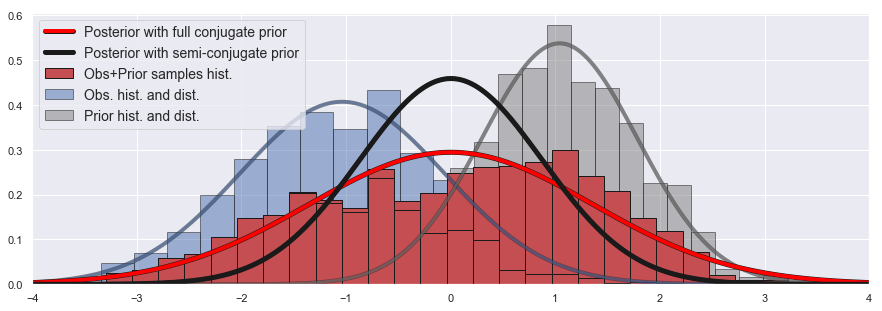
\includegraphics[width=\textwidth]{./Fig/LowRes/Full_vs_Semi_conjugate.png}
%     \caption{A comparison of the MLE estimations of the mean and variance for a single one dimensional Gaussian distribution (no prior), semi-conjugate prior and full conjugate prior MAPs. We have observed samples in blue, along with their estimated MLE Gaussian distribution, and a prior distribution in gray. Using confidence values of unity in the prior is similar to having an equal number of samples from the prior and in the observed data sets. A synthetic prior sample set is represented as the gray histogram. The posterior distribution with a semi-conjugate prior is in black and is seen as an average of the parameters of the observed and prior distributions. The posterior distribution with a full conjugate prior is in red. The red histogram is obtained by merging the observed samples with the synthetic prior samples. This histogram corresponds to the posterior distribution with a full conjugate prior. Note that the variance is larger than for either of the two original distributions; this results because of  the difference in the means. Legend: Hist. stands for histogram; Dist. stands for distribution; Obs. stands for observed samples.}
%     \label{Full_vs_Semi_conjugate}
% \end{figure*}

% In this section, we elaborate on the difference between a full and a semi-conjugate prior approach for estimating the parameters of a single, one dimensional, Gaussian distribution. After giving the needed definitions for the full conjugate prior and how the MAP-EM updates are affected, we illustrate the difference between semi and full conjugate through the example displayed in Fig. \ref{Full_vs_Semi_conjugate}.

% We first need some definitions. The full conjugate prior for the mean and variance follows a Normal-Inverse-Gamma distribution \citep{Murphy:2012:MLP:2380985}. As in section \ref{UpdateTheta}, we use the Normal-Inverse Chi-Squared re-parameterization:

% \begin{align}
% &\mathcal{P}({\mu},\sigma^2) = \mathcal{N}\mathcal{X}^{-2}({\mu}, \sigma^2|{\mu}_{prior}, K, N,\sigma_{prior}^2) \label{mu_sigma_prior}
% \end{align}
% With the confidences $K$ in the prior mean and $N$ in the prior variance:
% \begin{align}
% &{K}=({\kappa}{\pi}_{prior}V)^{-1}\\
% &{N}={\nu}{\pi}_{prior}V
% \end{align}

% The update of the means in MAP-EM algorithm stays the same as for the semi-conjugate prior approach, as detailed in equation \ref{mu_update}. On the contrary the update of the variances now requires an additional term ${s_{\bar{{\mu}}}}_j^{(k)}$ to account for the difference between the observed and the prior means:

% \begin{align}
% &{\sigma_j^2}^{(k)} = \frac{{{V_{j}^{(k)}} {\sigma^2_{\bar{\mathbf{m}}}}_j}^{(k)} + \nu_j {\pi_j}_{prior} V {\sigma_j^2}_{prior}+ {s_{\bar{{\mu}}}}_j^{(k)} }
% {{V_{j}^{(k)}} + \nu_j {\pi_j}_{prior} V} \label{sig_update_full}\\
% &\text{with:} \nonumber\\
% &{\sigma^2_{\bar{\mathbf{m}}}}_j^{(k)} =\frac{1}{{V_{j}^{(k)}}} \sum_{i=1}^{n} v_i n_{ij}^{(k)}({m}_i-\bar{{m}_j}^{(k)})^2\\
% &{s_{\bar{{\mu}}}}_j^{(k)} = \frac{\kappa_j V_{j}^{(k)} }{\kappa_j + V_{j}^{(k)}}(\bar{{m}}_j^{(k)}-{{\mu}_{j}}_{prior})^2 \label{full_additionalterm}
% \end{align}

% We illustrate those concepts with Fig. \ref{Full_vs_Semi_conjugate}. Let us consider the following setup. We have a set of observations (in our framework, this was our geophysical model), represented through their histogram in blue. The Gaussian distribution in blue represents the MLE parameters (estimated without any prior information). We now add prior information in the form of a Gaussian distribution, in gray in the Fig. \ref{Full_vs_Semi_conjugate}. We set the confidence parameters $\kappa$ and $\nu$ to unity, meaning that we have equal confidence in the observations and the prior ($\zeta$ is irrelevant here as we have only one Gaussian distribution). This equal confidence can be represented by having an equal number of samples from the prior than in the observed set. The histogram of this prior synthetic samples set set is shown in gray.

% The full conjugate prior approach can be understood as fitting a Gaussian distribution on the dataset formed by merging the observed and synthetic observations; this is represented in Fig. \ref{Full_vs_Semi_conjugate} in red. The full conjugate MAP distribution, also in red, is well centered between the two observed and prior distribution as expected, and so is the semi-conjugate distribution (in black). However the variance of the red histogram, and thus of the posterior distribution with full conjugate prior, is higher than the variance of either the observed or prior distribution. This is due to the difference in the means of the two distributions, which the full conjugate prior approach accounts for (see equations \ref{sig_update_full} and \ref{full_additionalterm}). The semi-conjugate prior approach considers the means and variances independently (see equations \ref{mu_semiprior} and \ref{sigma_semiprior}). The MAP mean estimates are the same for both priors.

% The semi-conjugate prior approach seems a better choice in the context of geophysical inversion. As our goal with this framework is to differentiate various geological units, by guiding the geophysical model to reproduce certain features, the full conjugate prior approach is sometimes detrimental as it can drive the variance further from the prior than what is currently seen in the model at each iteration.


% %%%%%%%%%%%%%%%%%%%%%%%%%%%%%%%%%%%%%%%%%%%%%%%%%%%%%%%%%%%%%%%%%%%%%%%%%%%%%%%
% \appendix{Pseudocode algorithm} \label{section:pseudocode}

% \begin{algorithm*}[ht!]
%     %\setstretch{1}
%     \SetKwInOut{Initialization}{Initialization}
%     \caption{This algorithm finds a geophysical model reproducing the geophysical, petrophysical and geological data.}
%     \label{algo:algorithm}
%     \nl \Initialization{
%     \begin{itemize}
%     \item \underline{Input:}
%     \begin{itemize}
%         \item Initial geophysical model $\mathbf{m}^{(0)}$, petrophysical distributions $\Theta^{(0)}$ and geological model $\mathbf{z}^{(0)}$.
%     \end{itemize}

%     \item \underline{Parameters:}
%     \begin{itemize}
%       \item \textit{Objective function}: data's noise matrix $W_d$, trade-off parameter $\beta^{(0)}$, prior matrices and weights $\left\{\alpha\right\}$, ${\left\{W\right\}}$.
%       \item \textit{Localized prior}: specific $\mathcal{P}(z_i)$ for available locations $i \in \{1..n\}$, local weights $\left\{\mathbf{w}_{i}\right\}_{i=1..n}$.
%       \item \textit{Confidences in the petrophysical prior}: $\left\{\kappa_j,\nu_j,\zeta_j\right\}_{j=1..c}$ for the means, variances and global proportions.
%       \item \textit{Optimization}: $\beta$-cooling factor $\gamma$ ($> 1$), sufficient decrease rate $\tau$ ($\leq 1$).
%     \end{itemize}

%     \item \underline{Output:}
%     \begin{itemize}
%         \item $\mathbf{m}$, $\Theta$, $\mathbf{z}$.
%     \end{itemize}

%     \end{itemize}
%     }

%     \While{${\Phi_d}>{\Phi_d^*}$ and $\Phi_s>\Phi_s^*$}{

%         \underline{Objective-Function Descent Step:}
%         \begin{itemize}
%         \item Compute a model perturbation $\delta \mathbf{m}$ for \ref{tikhonov} with the smallness defined in \ref{smallness_petro} using an inexact Gauss-Newton approach.
%         \item Backtracking line search with a Wolfe condition to find a step-size $\eta$ that satisfy a sufficient decrease of the objective function.
%         \item Return $\mathbf{m}^{(t)} = \mathbf{m}^{(t-1)}+\eta \delta \mathbf{m}$.
%         \end{itemize}

%         \nl \underline{Update Petrophysical Distribution}
%         \begin{itemize}
%         \item Fit a new GMM $\Theta^{(t)}$ on $\mathbf{m}^{(t)}$ with a confidence in the prior determined by the hyper-parameters $\left\{\zeta\right\}$, $\left\{\kappa\right\}$, $\left\{\nu\right\}$ such as in equations \ref{pi_update}, \ref{mu_update} and \ref{sig_update} until no sufficient increase of \ref{theta_posterior} is observed.
%         \end{itemize}

%         \nl \underline{Classification:}
%         \begin{itemize}
%         \item Compute the membership $\mathbf{z}^{(t)}$ of the current model $\mathbf{m}^{(t)}$ as in equation \ref{membership} using $\Theta^{(t)}$ as the classifier.
%         \item Update $\mathbf{m}_{\text{ref}}$ and $W_s$ according to \ref{mref_update} and \ref{Ws_update} respectively using $\mathbf{z}^{(t)}$.
%         \end{itemize}

%         \nl \underline{Update weights:}\\
%         \uIf{$\Phi_d^{(t)}>\Phi_d^*$ and $\Phi_d^{(t)}>\tau \Phi_d^{(t)}$}{
%             \begin{itemize}
%             \item Decrease $\beta$: $\beta^{(t)}=\frac{\beta^{(t-1)}}{\gamma}$
%             \end{itemize}
%         }
%         \uElseIf{$\Phi_d^{(t)}\leq\Phi_d^*$ and $\Phi_s>\Phi_s^*$}{
%             \begin{itemize}
%             \item Increase $\alpha_s$: $\alpha_s^{(t)}=\alpha_s^{(t-1)} \times \frac{{\Phi_d^*}}{{{{\Phi_d}}^{(t)}}}$
%             \end{itemize}
%         }
%         \uIf{(optional) $\Phi_d^{(t)}\leq\Phi_d^*$ and $\Phi_s>\Phi_s^*$ and $\mathbf{z}^{(t)}==\mathbf{z}^{(t-1)}$}{
%             \begin{itemize}
%             \item Include $\mathbf{m}_{\text{ref}}$ in Smoothness
%         \end{itemize}
%         }
%     }
% \end{algorithm*}

% We give in algorithm $1$ the details of our implementation of this framework. The optimization notions of inexact Gauss-Newton and backtracking line search are detailed in \cite{Ascher2011}, or in \cite{haber2014computational} for their geophysical applications.

% Figure ~\ref{Flowchart} graphically summarizes in a flowchart how our framework loops over the various datasets to produce a final geophysical model with the desired petrophysical distribution and geological features.

% \begin{figure}
%     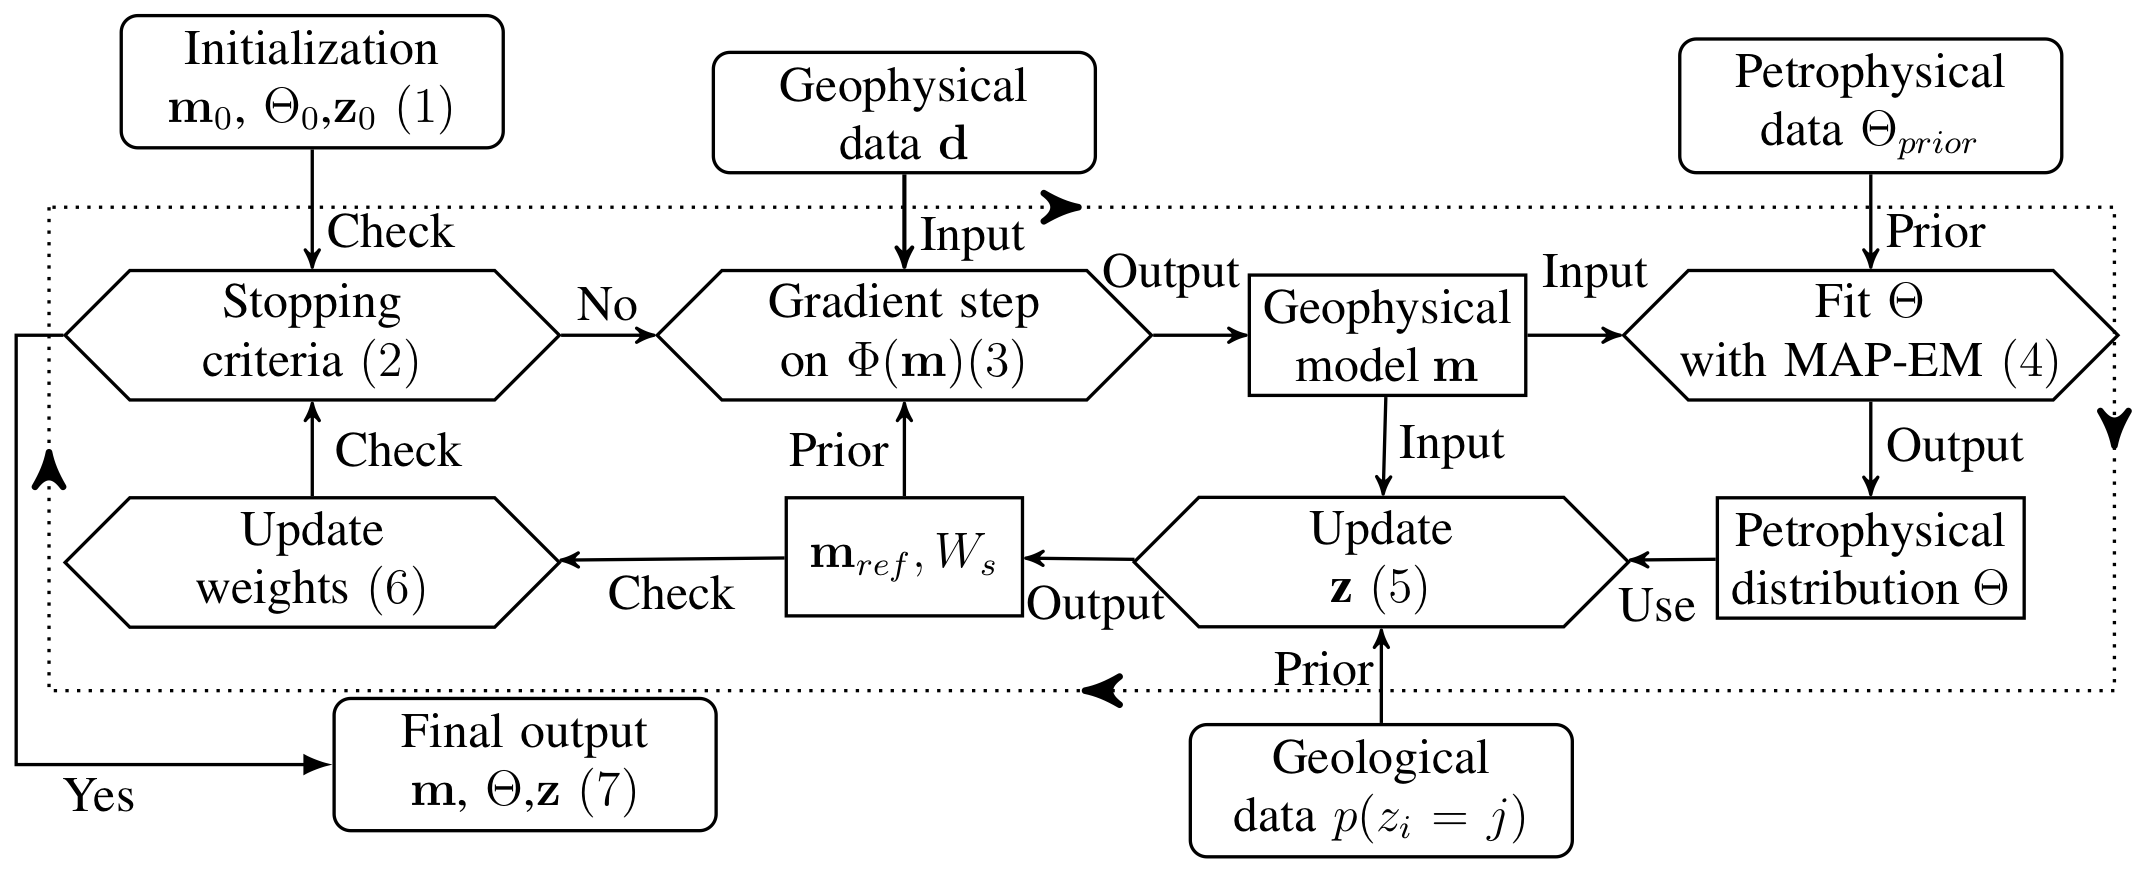
\includegraphics[width=\columnwidth]{./Fig/LowRes/Flowchart.png}
%     \caption{A visual pseudocode of our iterative cyclic framework to include geological and petrophysical information into geophysical inversion. The numbers correspond to the steps displayed in algorithm 1.}
%     \label{Flowchart}
% \end{figure}

% \label{lastpage}

\end{document}
